\documentclass{article}\usepackage{knitr}

\usepackage{setspace}
\usepackage{booktabs}
\linespread{1.25}

%% Luk_pohja.tex-tiedostosta
%% Oma sivukoko
\setlength{\textheight}{9in}
\setlength{\textwidth}{6in}
\setlength{\topmargin}{0in}
%% Tekstialueen keskitys sivulle (arvot löydetty kokeilemalla)
\setlength{\oddsidemargin}{0.4cm}
\setlength{\evensidemargin}{0.4cm}

\usepackage{bm}
\usepackage{url}
\usepackage{amsmath}
\usepackage{interval}
\usepackage{setspace}
\usepackage{multirow}
\usepackage{graphicx}
\usepackage{float}

\graphicspath{ {./figures/} }

\usepackage[T1]{fontenc}
\usepackage[finnish, english]{babel}
\usepackage[utf8]{inputenc}

\onehalfspacing
\usepackage[natbibapa, nodoi]{apacite}
\usepackage{tcolorbox}

\usepackage{algorithm}
\usepackage[noend]{algpseudocode}





\IfFileExists{upquote.sty}{\usepackage{upquote}}{}
\begin{document}

\thispagestyle{empty}

\thispagestyle{empty}
\begin{center}
\null\vspace{3cm}
\Large
Bayesian Inference and Adaptive Estimation in General Recognition Theory\\[2cm]
\large
Joni Pääkkö\\[1cm]
\vfill
\normalsize
\end{center}
\begin{flushright}
Maisterintutkielma\\
Jyväskylän Yliopisto\\
MUTKU\\ 
Kevät 2020
\end{flushright}

\newpage

\begin{abstract}

General Recognition Theory (GRT) is a multidimensional generalization of Signal Detection Theory. It is used to model the detection of signals with multiple dimensions, e.g. auditory signals which can vary not only in their pitch but also in their timbre independently. Main focus is in if the detection of these dimensions is coupled.

Bayesian adaptive estimation has been succesfully applied to many different tasks and models in psychophysics. The main goal of this thesis is to study the application of it to GRT models. To achieve this, I will introduce a GRT models for a Yes/No and 2I-4AFC procedure that include psychometric functions to model the relationship between physical signal strengths and $d'$ explicitly. Also, methods for Bayesian estimation of these models are introduced.

The performance of the models are evaluated in simulations (N = 772) and in a small scale psychophysical experiment (N = 2).

Simulations indicate that the adaptive algorithm is more efficent on average, but offers little practical improvement over random sampling in this context. 

Data from the psychophysical experiments indicate that non-sensory factors play a big part, indicating that more work should be put into developing models/procedures that can identify between these factors. The data also suggests that the often default choice of coupling means does not necessarily capture all relevant properties of it. 

\end{abstract}

\newpage

\tableofcontents

\newpage

\setcounter{page}{1}
\newpage

%!Rnw root = ../Main.Rnw

\section{Simulations}

I will be considering two main questions: 

\begin{enumerate}
  \item How much more efficient the adaptive algorithm is in relation to sampling stimuli from a fixed grid--if at all? 
  \item How well can generating parameters be recovered?
\end{enumerate}

These questions are closely related, since relative efficiency of the algorithms (Question 1) is defined here by the quantities that are also used to evaluate Question 2. 

There are two quantities of interest. First is defined by taking the means of the marginal posterior distributions as point estimates and calculating the squared differences to the generating parameters. This quantifies squared bias and variance of these estimators. The second quantity is the standard deviations of the marginal posterior distributions. This is used as a measure of how much uncertainty about the parameters is left after the data collection process. The goal, as already stated, is to minimize uncertainty about the parameters.

Question 1 is evaluated by inspecting if there are differences between the algorithms in how quickly the aforementioned quantities approach zero. Question 2 is answered by looking at the same  quantities, but the focus is on the overall performance, not differences. The first question is more closely related to the topic of this thesis, but the second question has more general value regarding the estimation of GRT models for which reason it can't be ignored. 

\subsection{Methods}

The general method was the following: first a set of generating parameters for the simulated observer were drawn randomly, and then either of the algorithms (adaptive/non-adaptive) described earlier were run. This was done for both the Yes/No and 21-4AFC procedure, resulting in four different conditions\footnote{There was a third algorithm, that consisted of sampling stimuli randomly from an adaptive grid, but results from this condition are not reported here, since it doesn't directly answer the main question posed in this thesis. The interested reader can find the data and R code to plot the results from: \url{https://github.com/joanpaak/Master_thesis}}. 

I have chosen the number 800 fairly arbitrarily; it represents a number of trials that, I think, could still be administered relatively continuously to a participant, without taking into account non-stationarities induced by a multi-session design. I have tried to pick a number that would b large enough; if one thinks that the number is lower, one can still get that information from the graphs. 

\paragraph{Prior distributions}

Prior distributions and distributions from which generating parameters for the simulations were drawn from are shown in Figure \ref{fig:priors} and in tabular form in Table \ref{tab:priors}. The same prior and generating distribution is used for both dimensions. Note that the scale for criterion is given in false alarm probabilities for easier interpretation. 

Priors for the parameters were chosen based on prior information from \citet{silbert2009} and from pilot testing. 

Prior for $\sigma$ was chosen to be fairly vague to reflect the possibility of widely differing thresholds.

Generating parameters for the simulations were drawn from bimodal distributions. The idea was to draw values that are covered by the prior, but which do not necessarily correspond with the mode of the prior distribution. Another motivation was to have qualitatively different simulated observers: some that have high values for some of the parameters and others that have low values.

\begin{figure}[!htb]
\centering
\begin{knitrout}
\definecolor{shadecolor}{rgb}{0.969, 0.969, 0.969}\color{fgcolor}
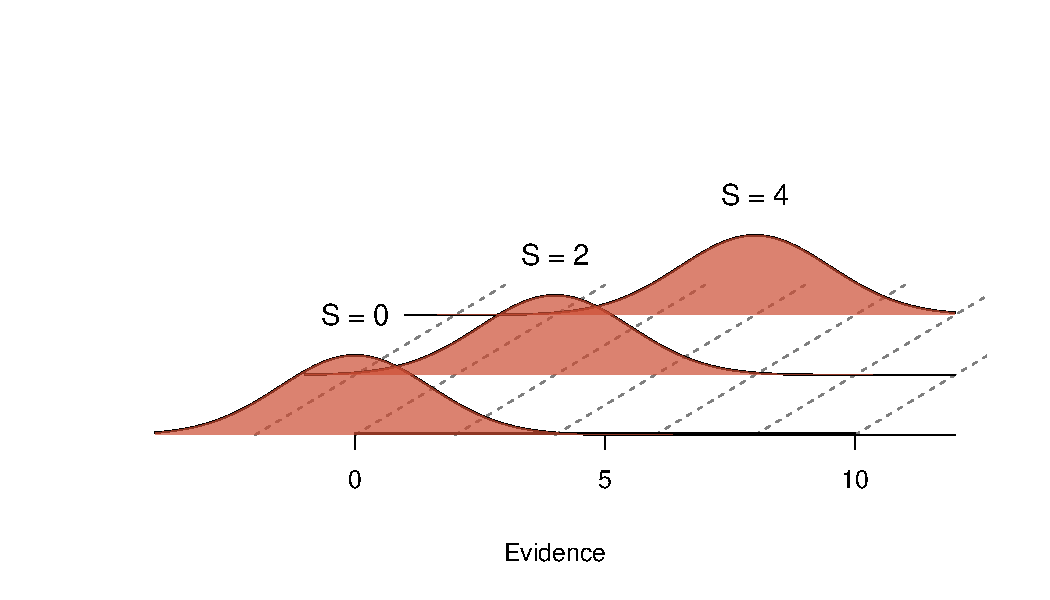
\includegraphics[width=\maxwidth]{figure/unnamed-chunk-2-1} 

\end{knitrout}

\caption{Prior distributions for the parameters of the model (solid black lines) and distributions for generating parameters for the simulations (regions shaded with red). Note that all of the densities are normalized to have maximum value of 1.0.}
\label{fig:priors}
\end{figure}

\begin{table}[H]
\centering
\caption{Parameters used for prior distributions and distributions of generating parameters. $M^l$ and $M^u$, respectively, are for the lower and upper peaks of bimodal distributions.}
\vspace{0.5cm}
\begin{tabular}{cccccc}
\toprule

          & \multicolumn{2}{c}{Prior} & \multicolumn{3}{c}{Generating}   \\
          \cmidrule(lr){2-3}\cmidrule(lr){4-6}
          & $M$       & $SD$    & $M^l$         & $M^u$         & $SD$   \\
\midrule
$\sigma$  & $log(2.5)$  & $0.75$   & $log(1)$    & $log(5)$    & $0.08$ \\
$C$       & $1.5$            & $0.3$   & $1.2$         & $1.7$         & $0.05$  \\
$\beta$   & $log(1)$  & $0.3$   & $log(0.8)$    & $log(1.2)$    & $0.05$ \\
$\kappa$  & $0$            & $0.3$   & $-0.25$        & $0.25$         & $0.075$ \\
$\rho$    & $0$            & $0.7$  & $atanh(0.75)$ & $atanh(-0.25)$  & $0.1$ \\
\bottomrule
\end{tabular}
\label{tab:priors}
\end{table}

\subsection{Results}

Total number of simulations per condition are shown in Table \ref{tab:conditions}. Squared errors and marginal standard deviations are presented in two ways: 1) on trial-by-trial basis and 2) by estimating the average differences on the last trial.

\begin{table}[H]
\centering
\caption{Conditions and number of simulations in each.}
\vspace{0.5cm}
\begin{tabular}{ccc}

\toprule
Procedure & Algorithm & N \\
\midrule
Yes/No & Adaptive & 184 \\
Yes/No & Random & 284 \\
2I-4AFC & Adaptive & 174 \\
2I-4AFC & Random & 130 \\

\bottomrule

\end{tabular}

\label{tab:conditions}
\end{table}

\paragraph{Trial-by-trial estimates}
Trial-by-trial results from the simulations are summarized in Figures \ref{fig:simulation_YN_sensory_sq_error} to \ref{fig:simulation_AFC_interaction_SD}. The figures show squared errors in relation to generating parameters and marginal standard deviations after $N$ trials, all the way to trial number 800. In all plots black color is used for the randomly sampled stimuli while red is used for adaptively sampled stimuli. The shaded regions indicate 50\%-quantiles (from 25\% to 75\%); solid lines indicate medians. Sensory ($\sigma$, $\beta$, crit) and interaction ($\kappa_{\mu}$, $\rho$) are shown in their own figures.

\begin{figure}[H]
\centering
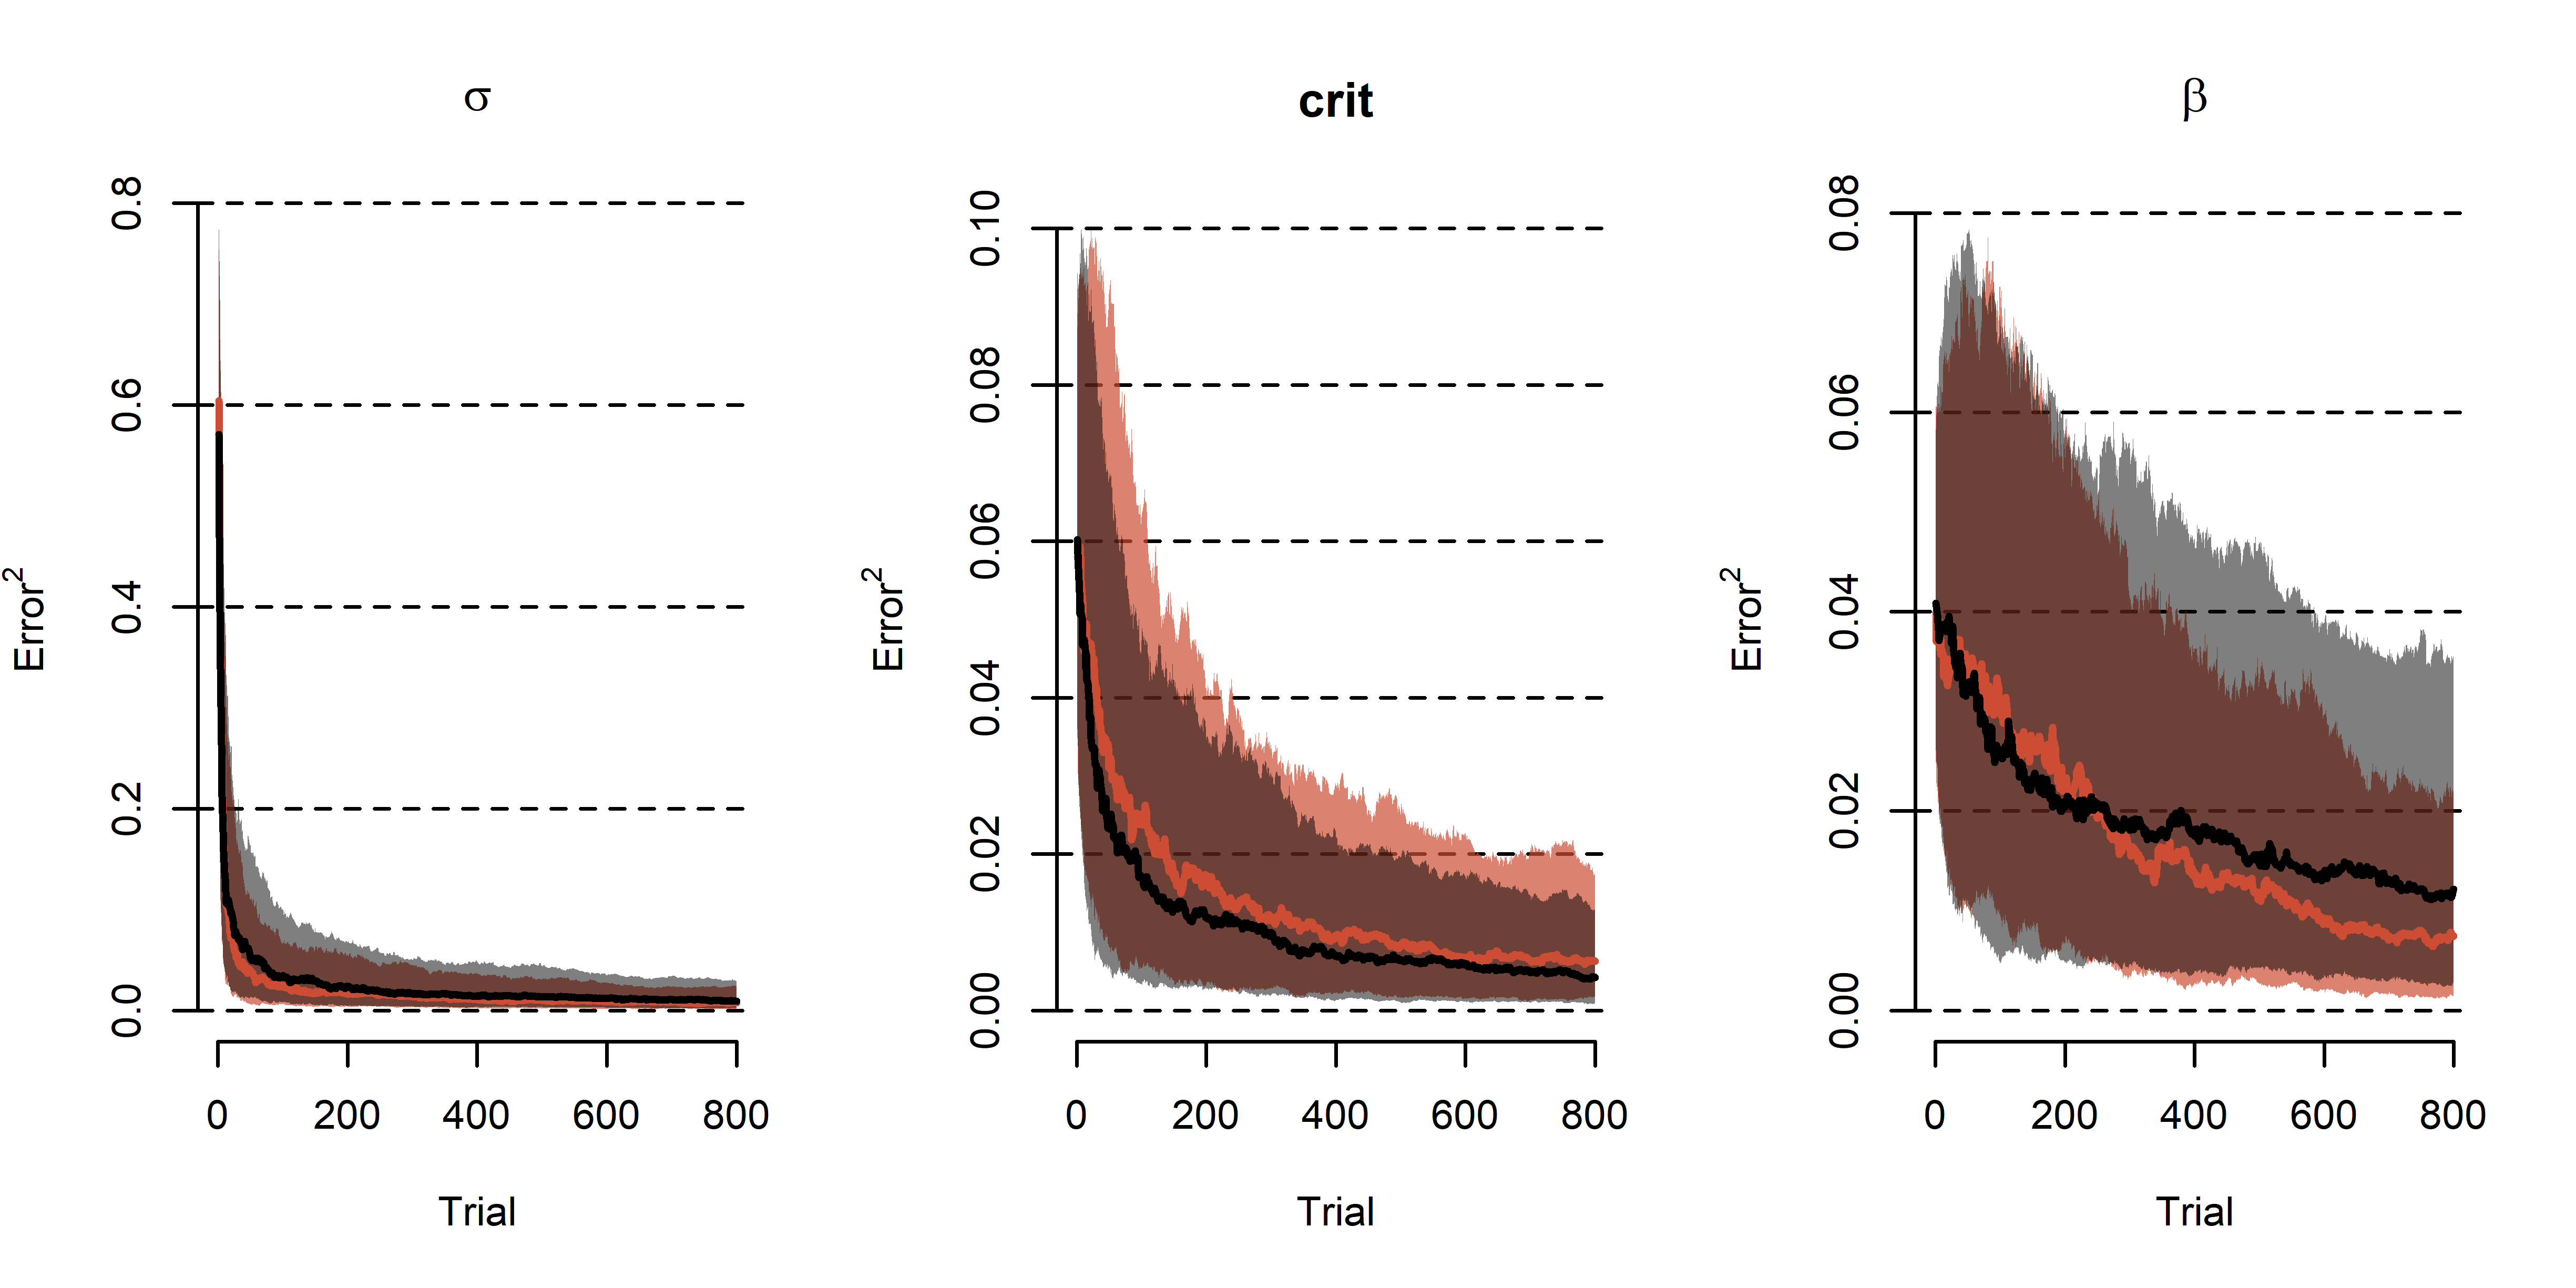
\includegraphics[scale=0.75, angle = 0]{simulation_YN_sensory_sq_error}
\caption{Procedure: Yes/No; sensory parameters. Trial-by-trial squared error between marginal means of the posterior distribution and generating parameters. Red: adaptive algorithm; black: random stimuli.}
\label{fig:simulation_YN_sensory_sq_error}
\end{figure}

\begin{figure}[H]
\centering
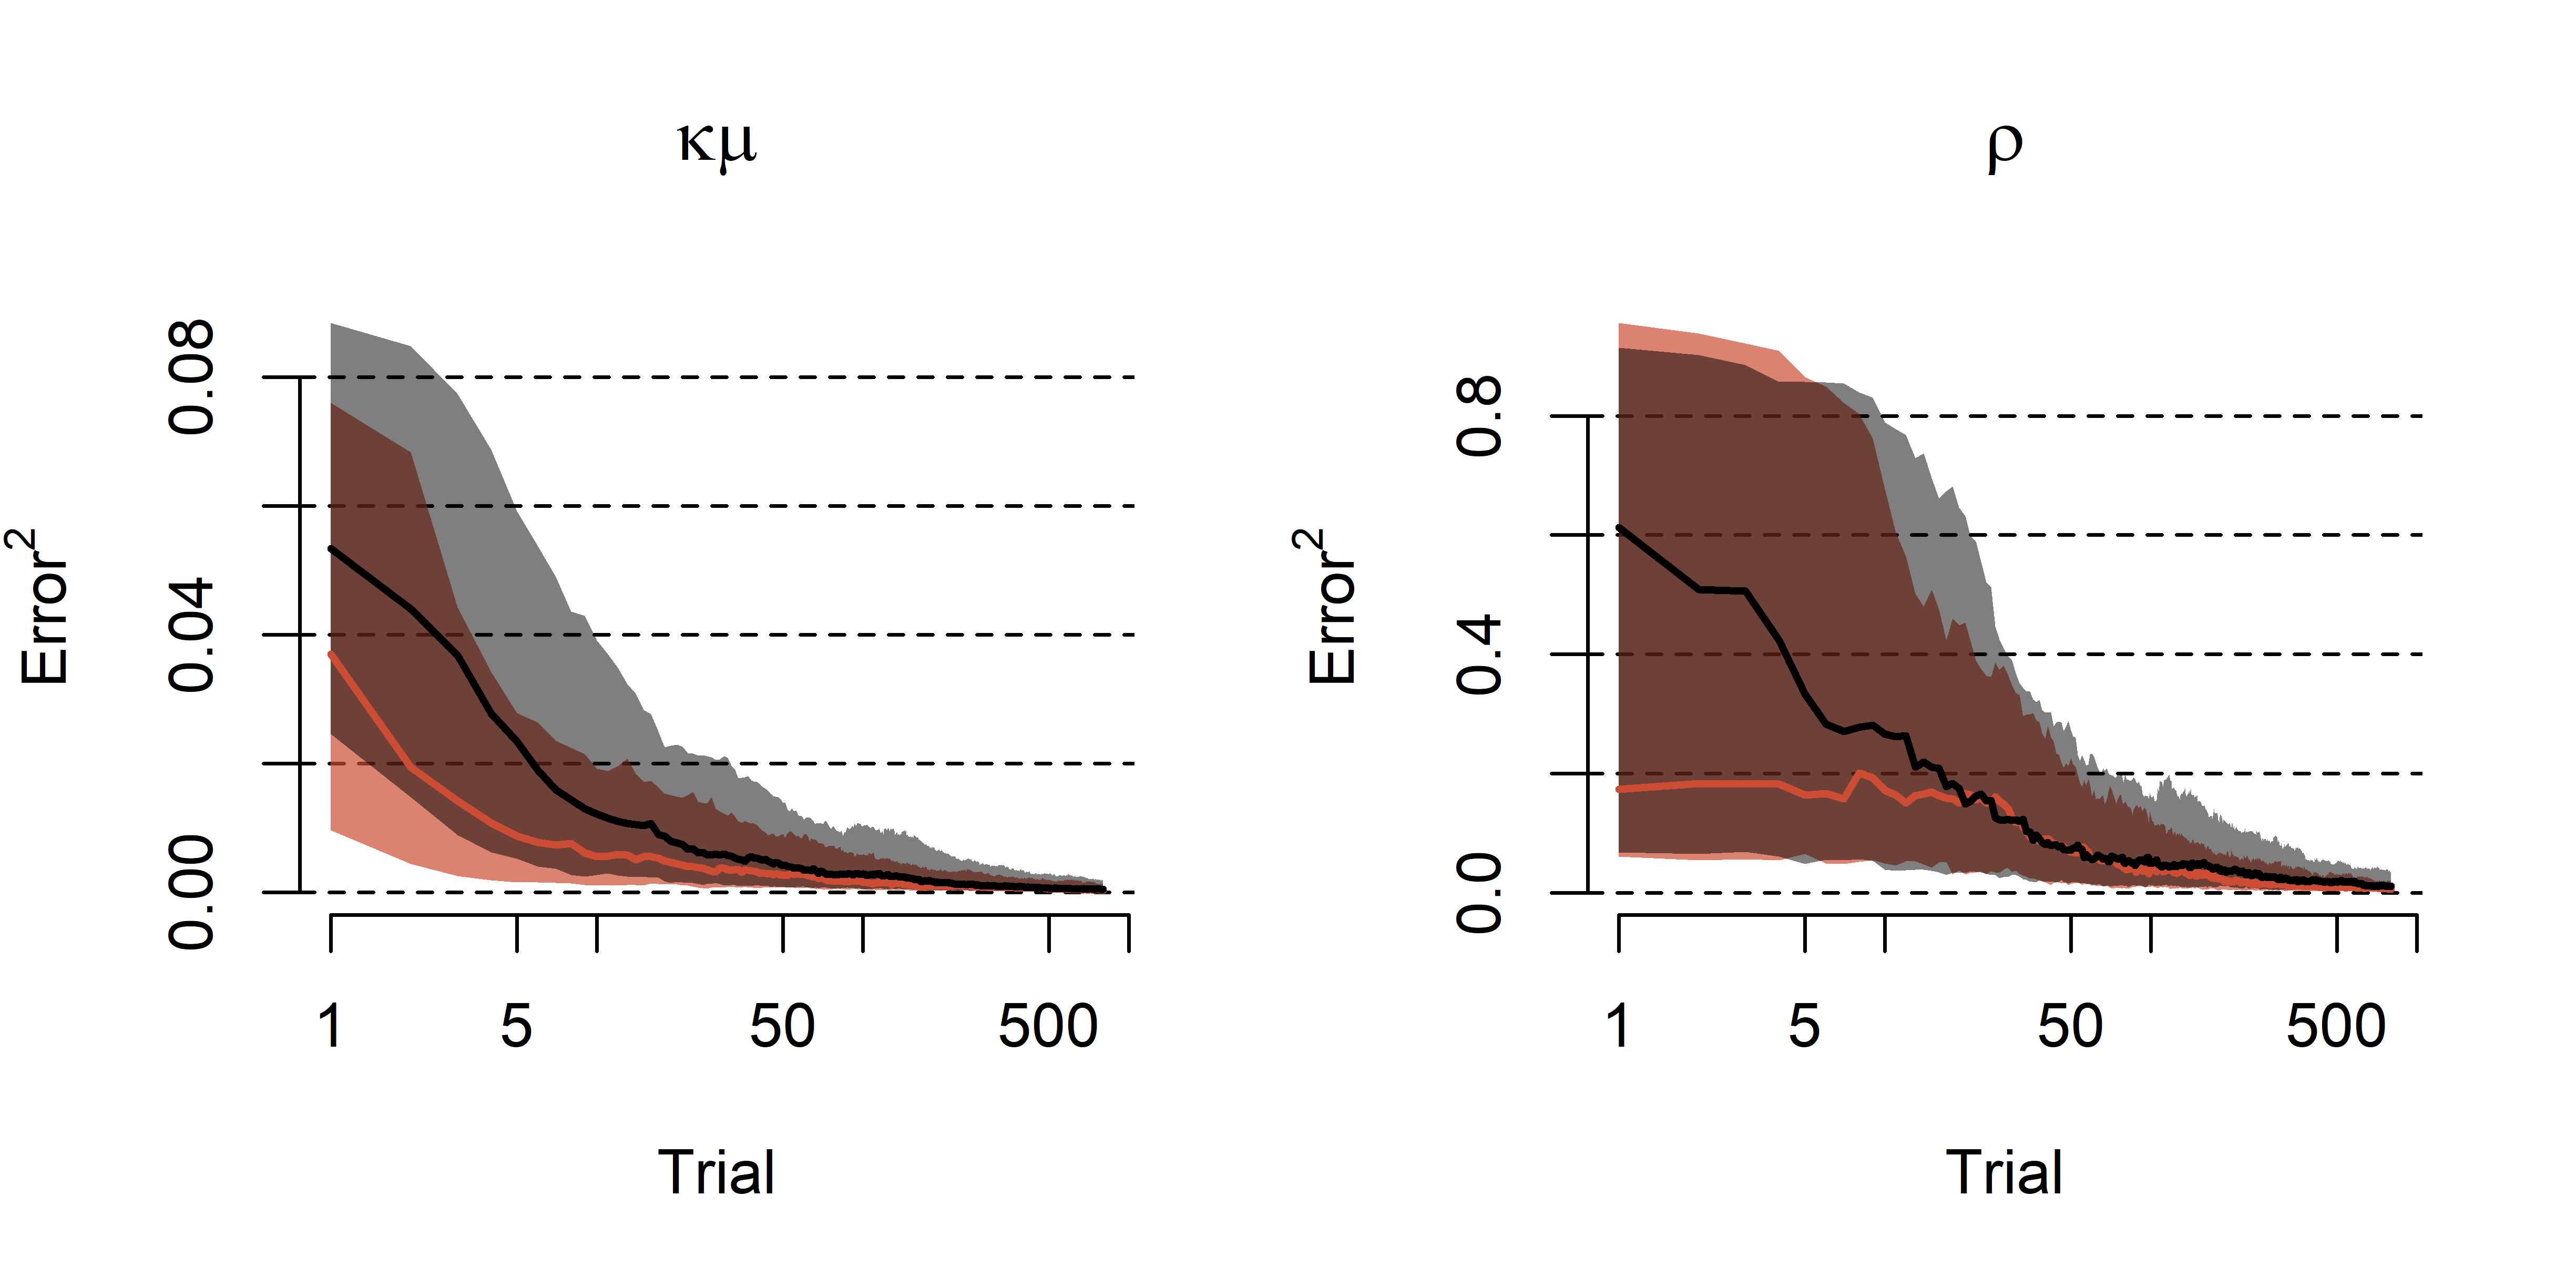
\includegraphics[scale=0.75, angle = 0]{simulation_YN_interaction_sq_error}
\caption{Procedure: Yes/No; interaction parameters. Trial-by-trial squared error between marginal means of the posterior distribution and generating parameters. Red: adaptive algorithm; black: random stimuli.}
\label{fig:simulation_YN_interaction_sq_error}
\end{figure}

\begin{figure}[H]
\centering
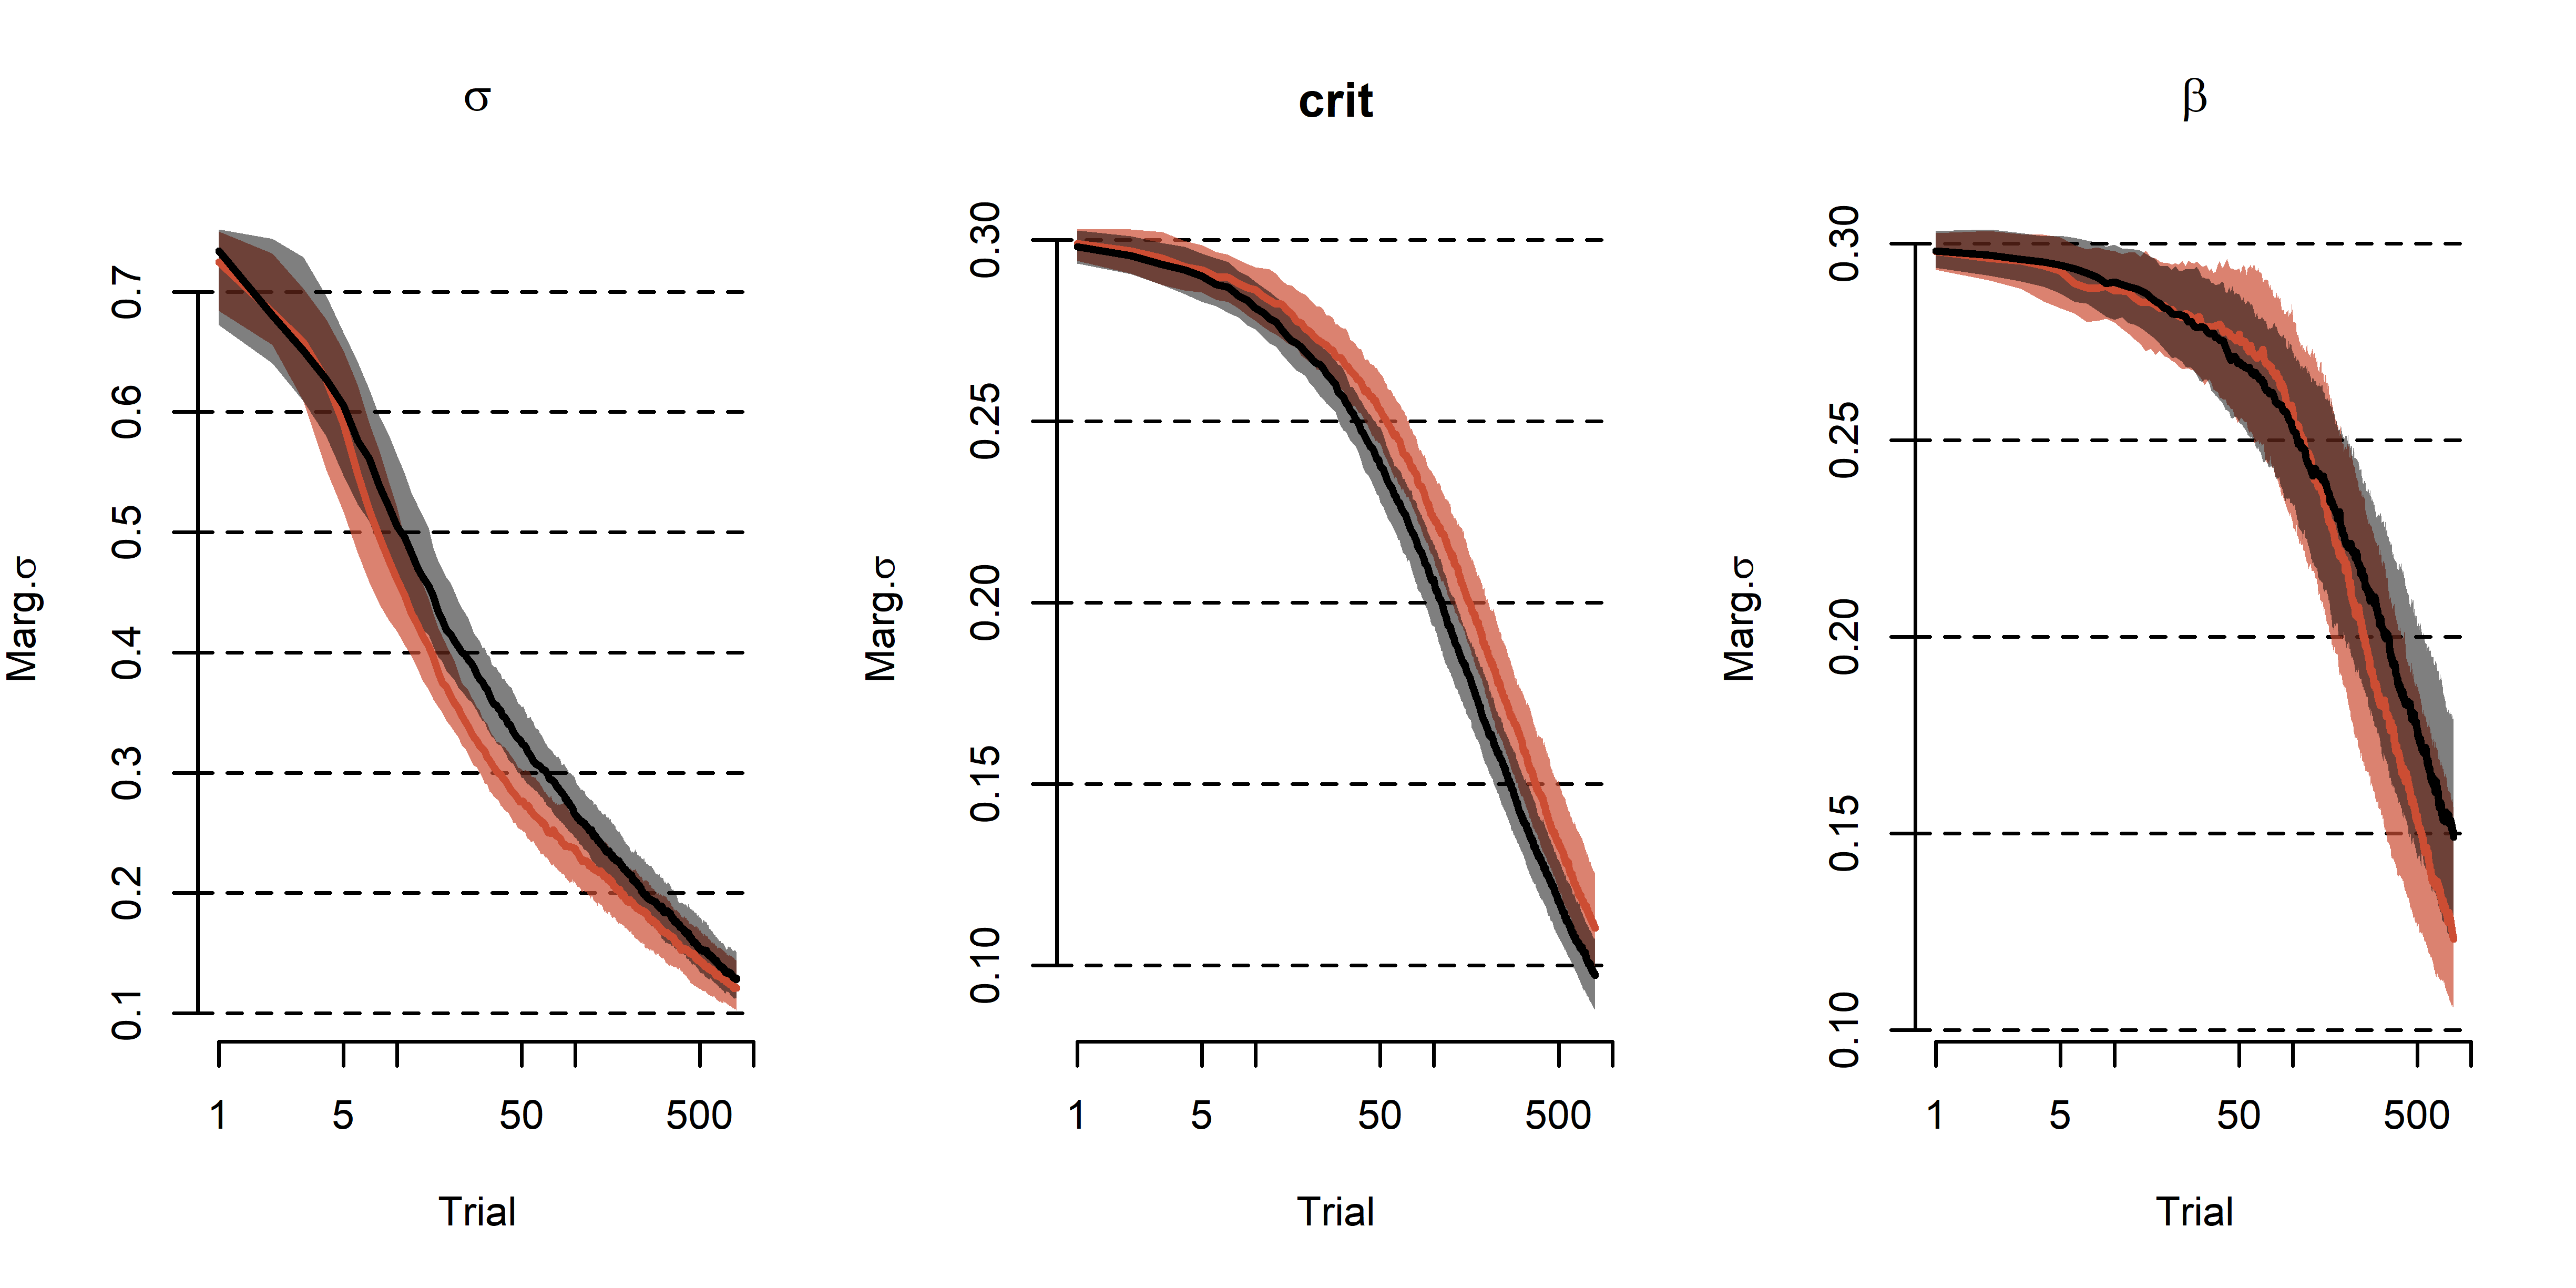
\includegraphics[scale=0.75, angle = 0]{simulation_YN_sensory_SD}
\caption{Procedure: Yes/No; sensory parameters. Trial-by-trial marginal standard deviations. Red: adaptive algorithm; black: random stimuli.}
\label{fig:simulation_YN_sensory_SD}
\end{figure}

\begin{figure}[H]
\centering
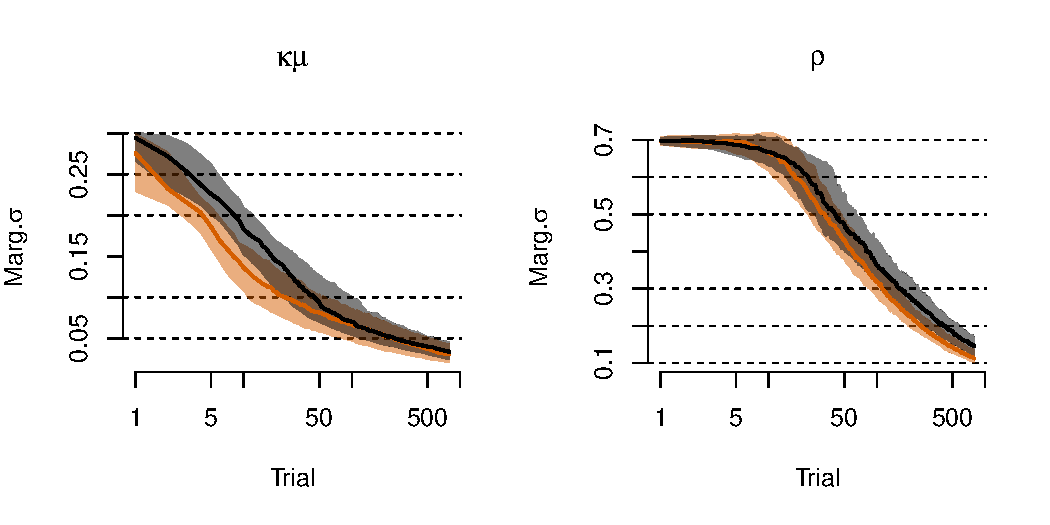
\includegraphics[scale=0.75, angle = 0]{simulation_YN_interaction_SD}
\caption{Procedure: Yes/No; interaction parameters. Trial-by-trial marginal standard deviations. Red: adaptive algorithm; black: random stimuli.}
\label{fig:simulation_YN_interaction_SD}
\end{figure}

\begin{figure}[H]
\centering
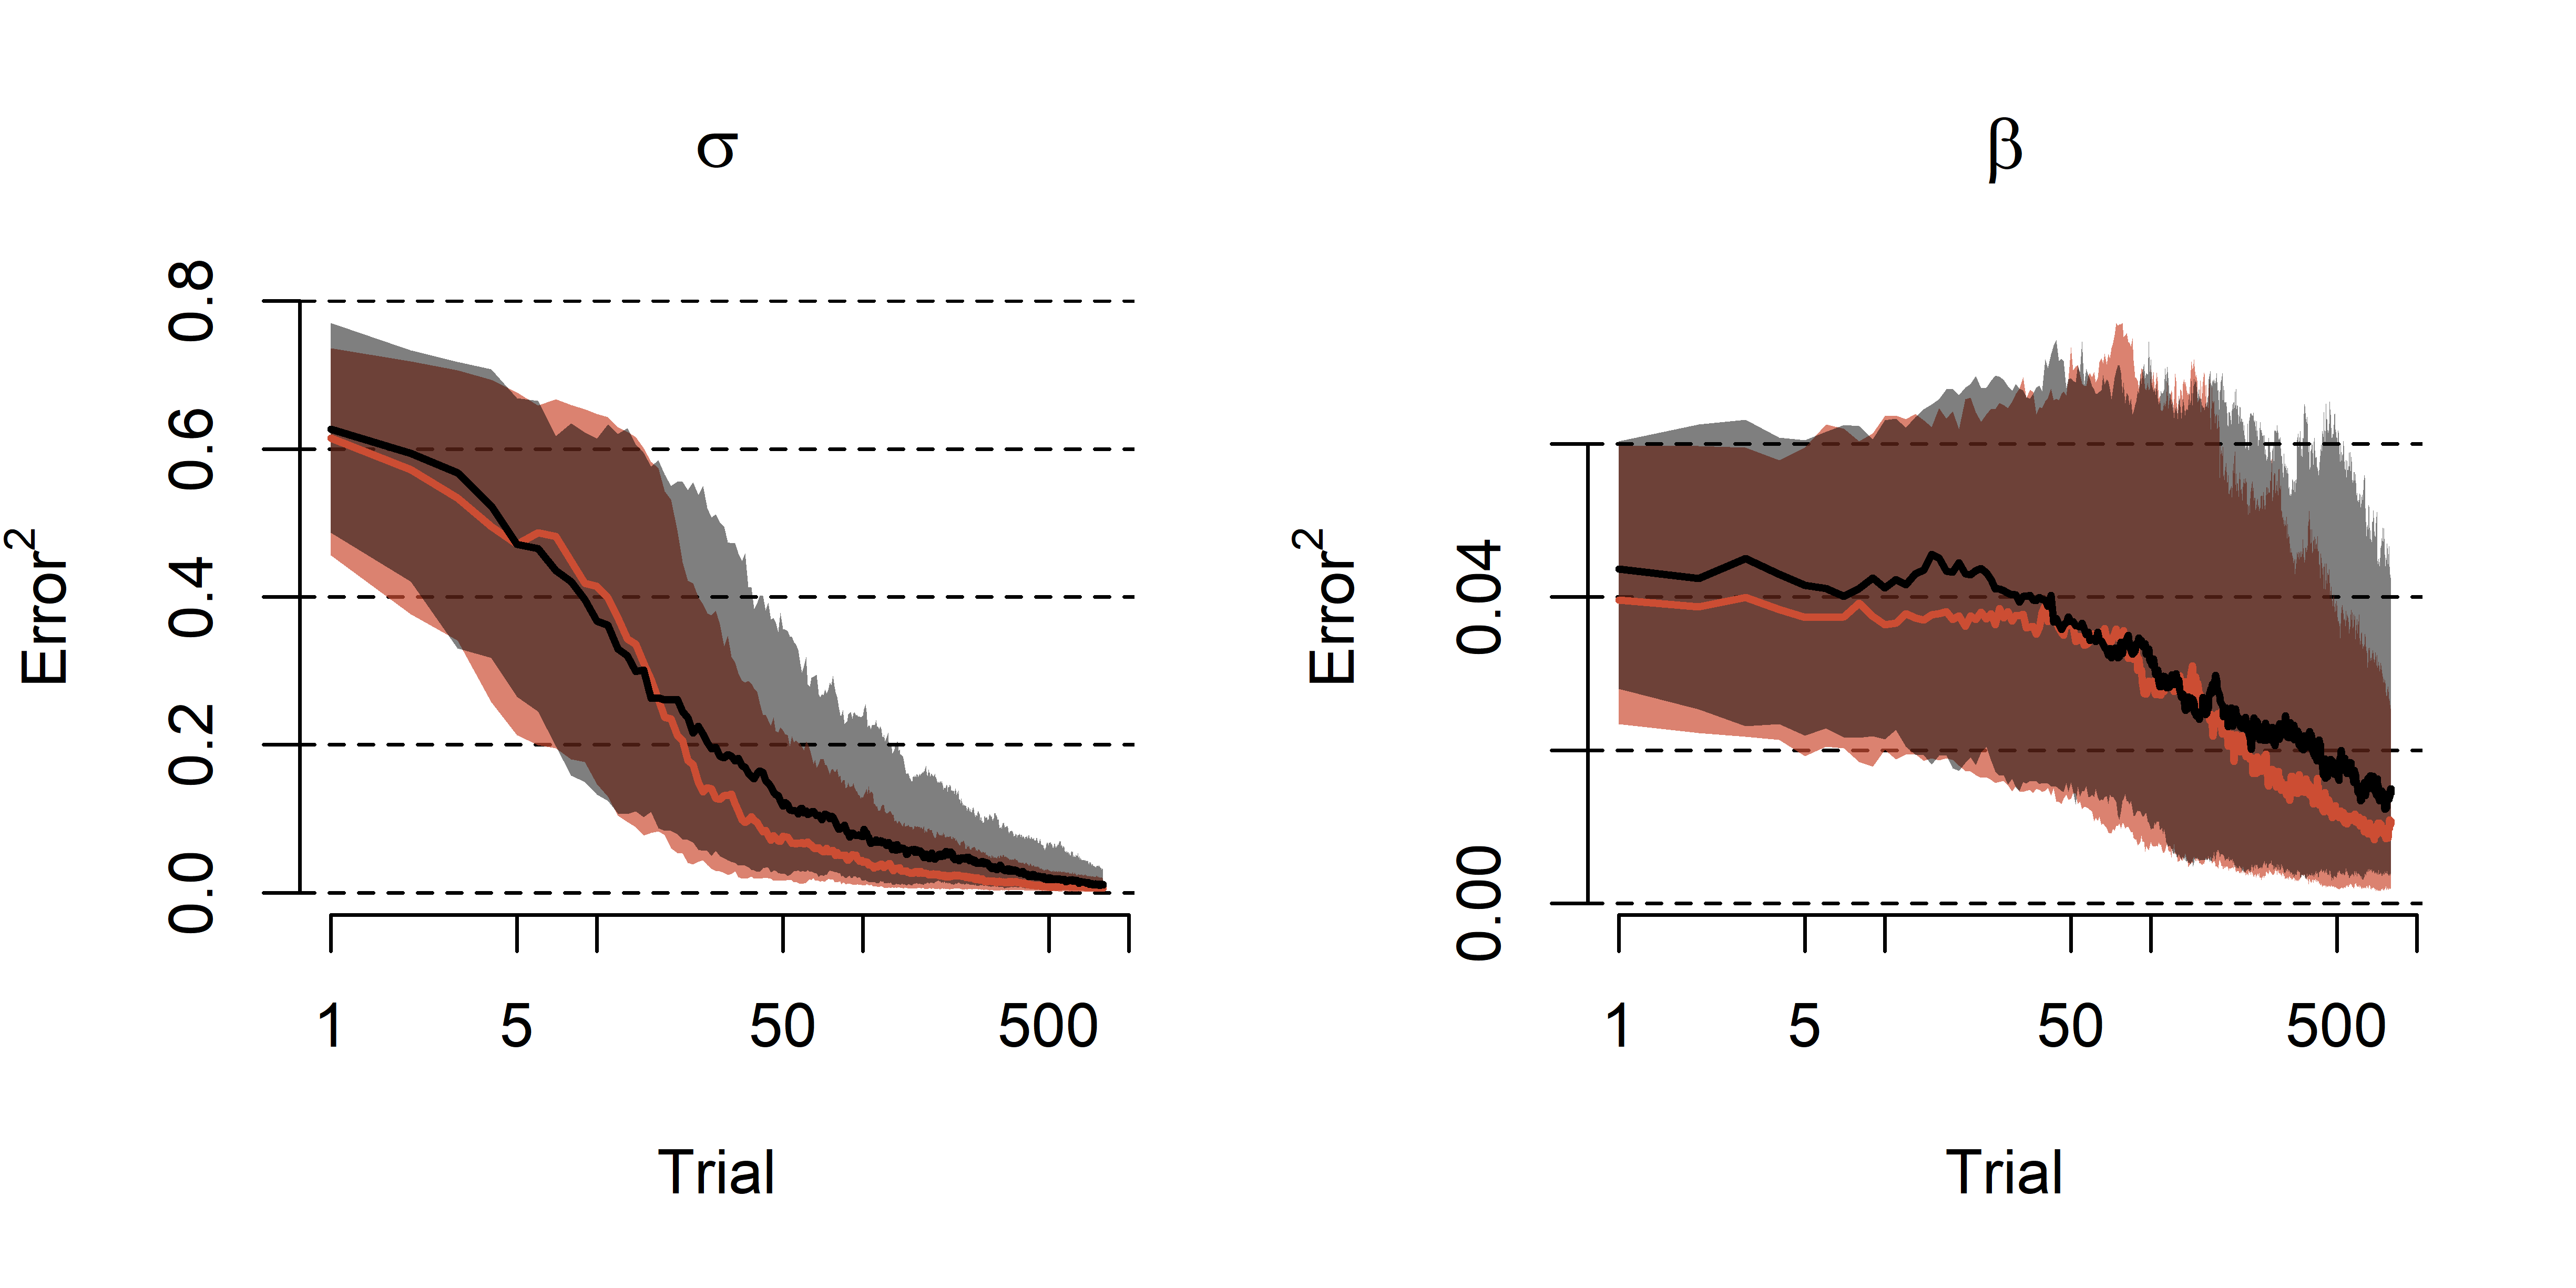
\includegraphics[scale=0.75, angle = 0]{simulation_AFC_sensory_sq_error}
\caption{Procedure: 2I-4AFC; sensory parameters. Trial-by-trial squared error between marginal means of the posterior distribution and generating parameters. Red: adaptive algorithm; black: random stimuli.}
\label{fig:simulation_AFC_sensory_sq_error}
\end{figure}

\begin{figure}[H]
\centering
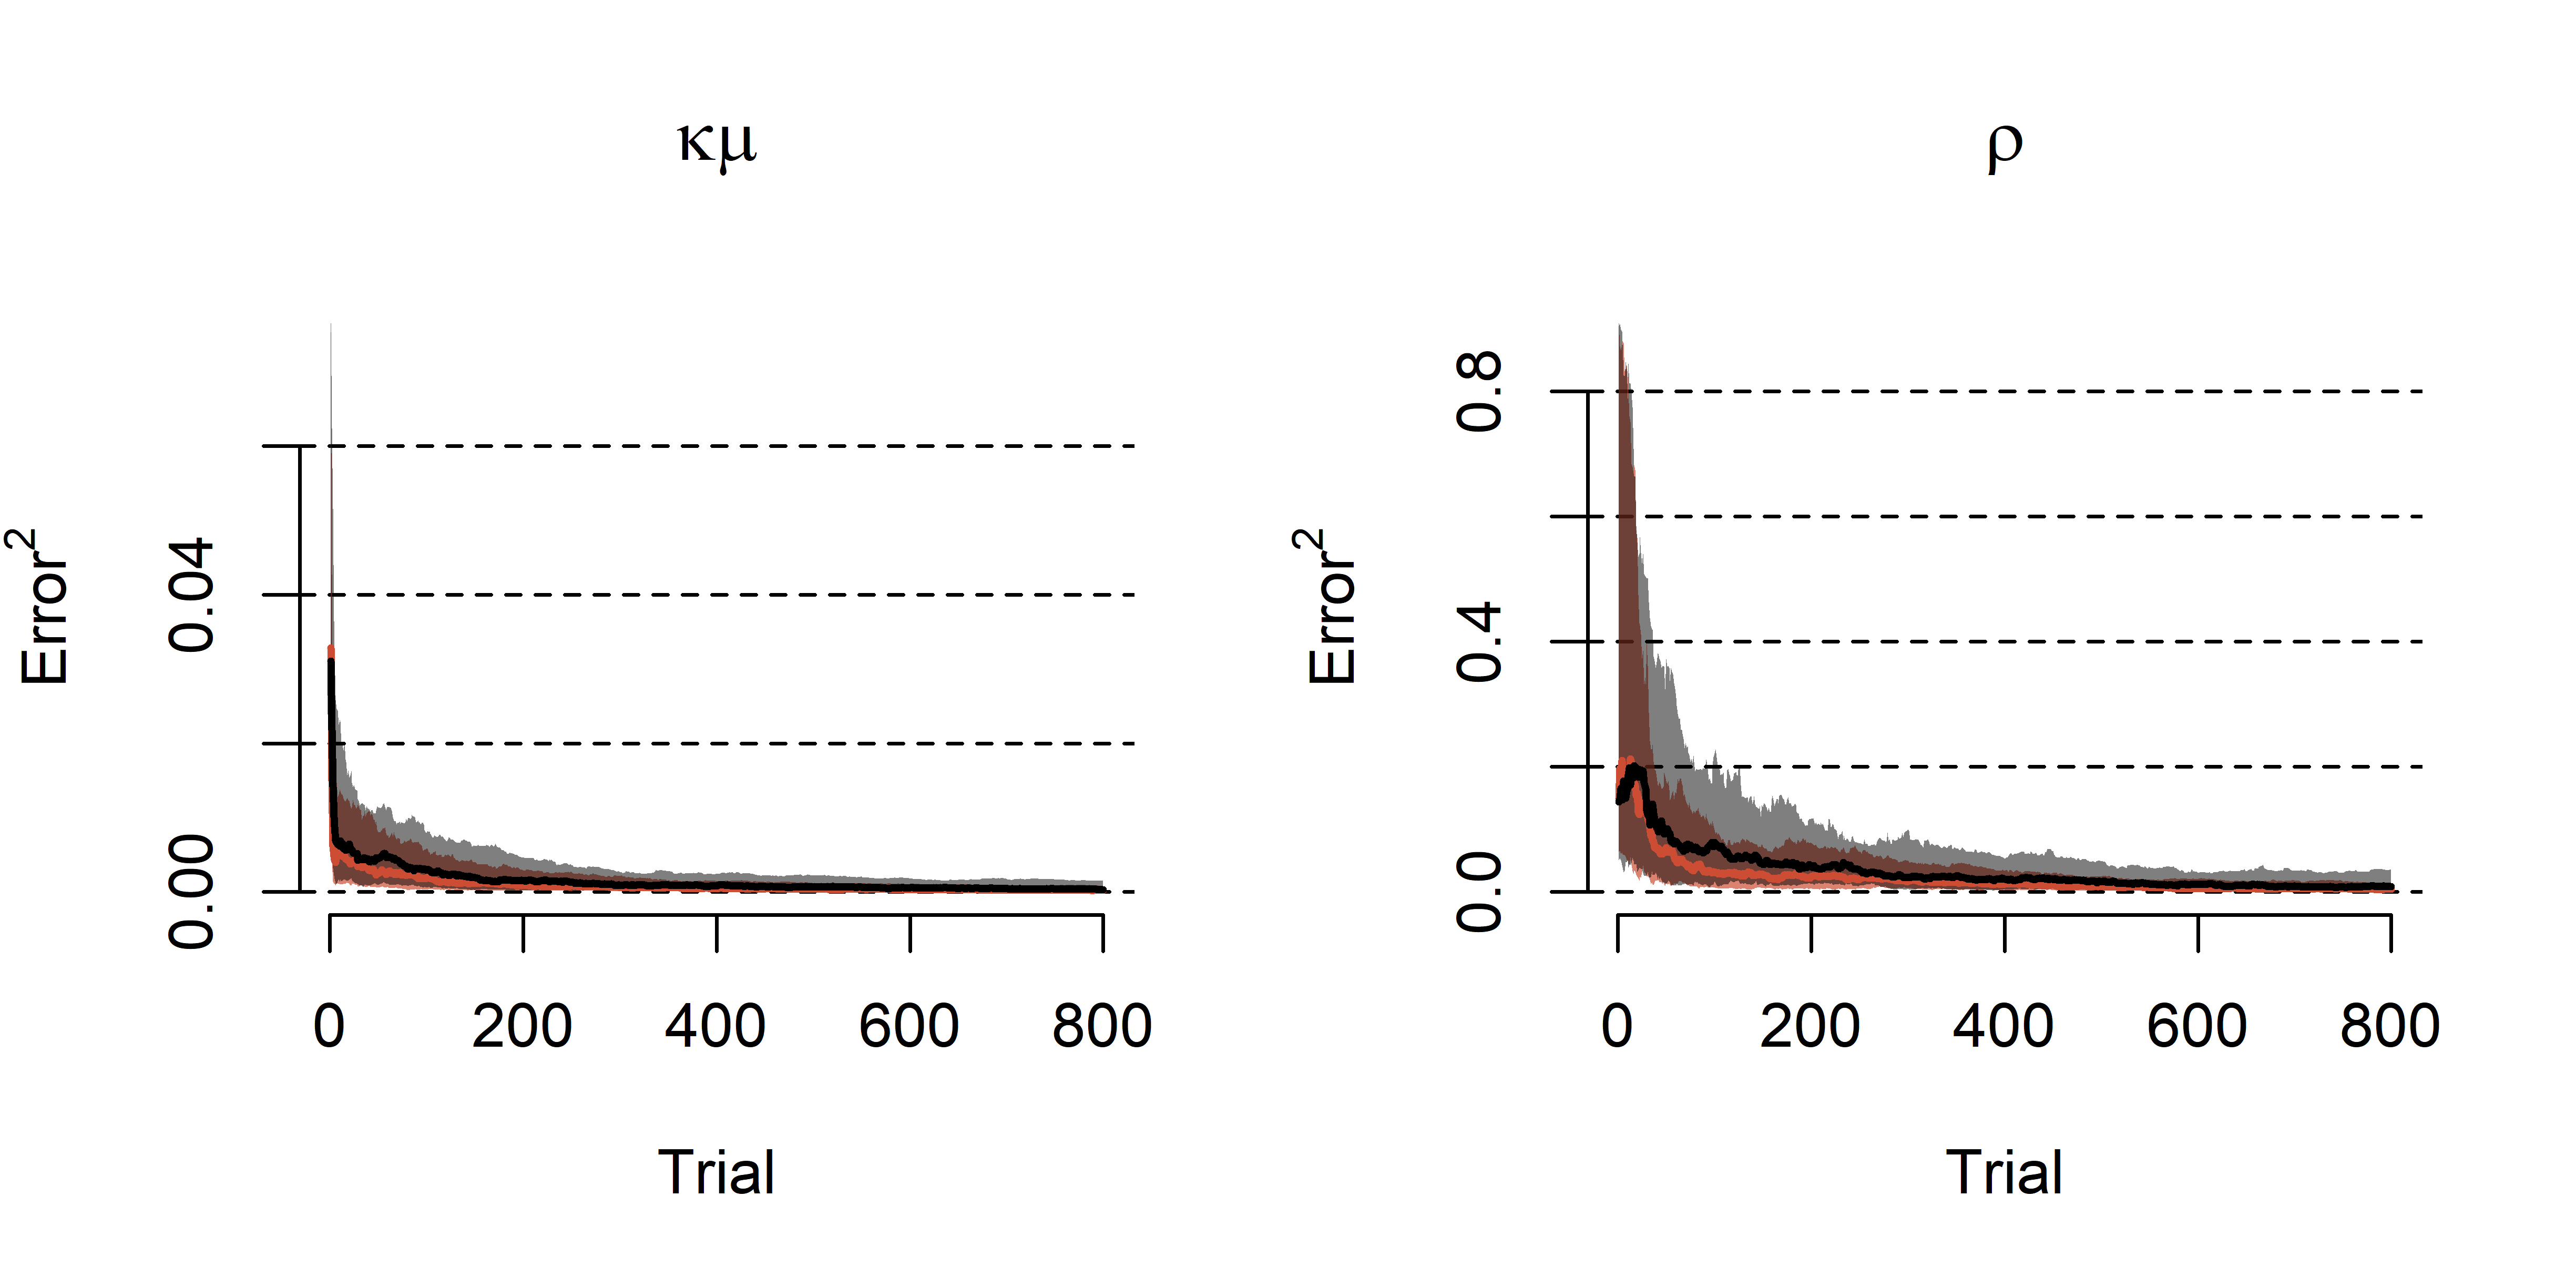
\includegraphics[scale=0.75, angle = 0]{simulation_AFC_interaction_sq_error}
\caption{Procedure: 2I-4AFC; interaction parameters. Trial-by-trial squared error between marginal means of the posterior distribution and generating parameters. Red: adaptive algorithm; black: random stimuli.}
\label{fig:simulation_AFC_interaction_sq_error}
\end{figure}

\begin{figure}[H]
\centering
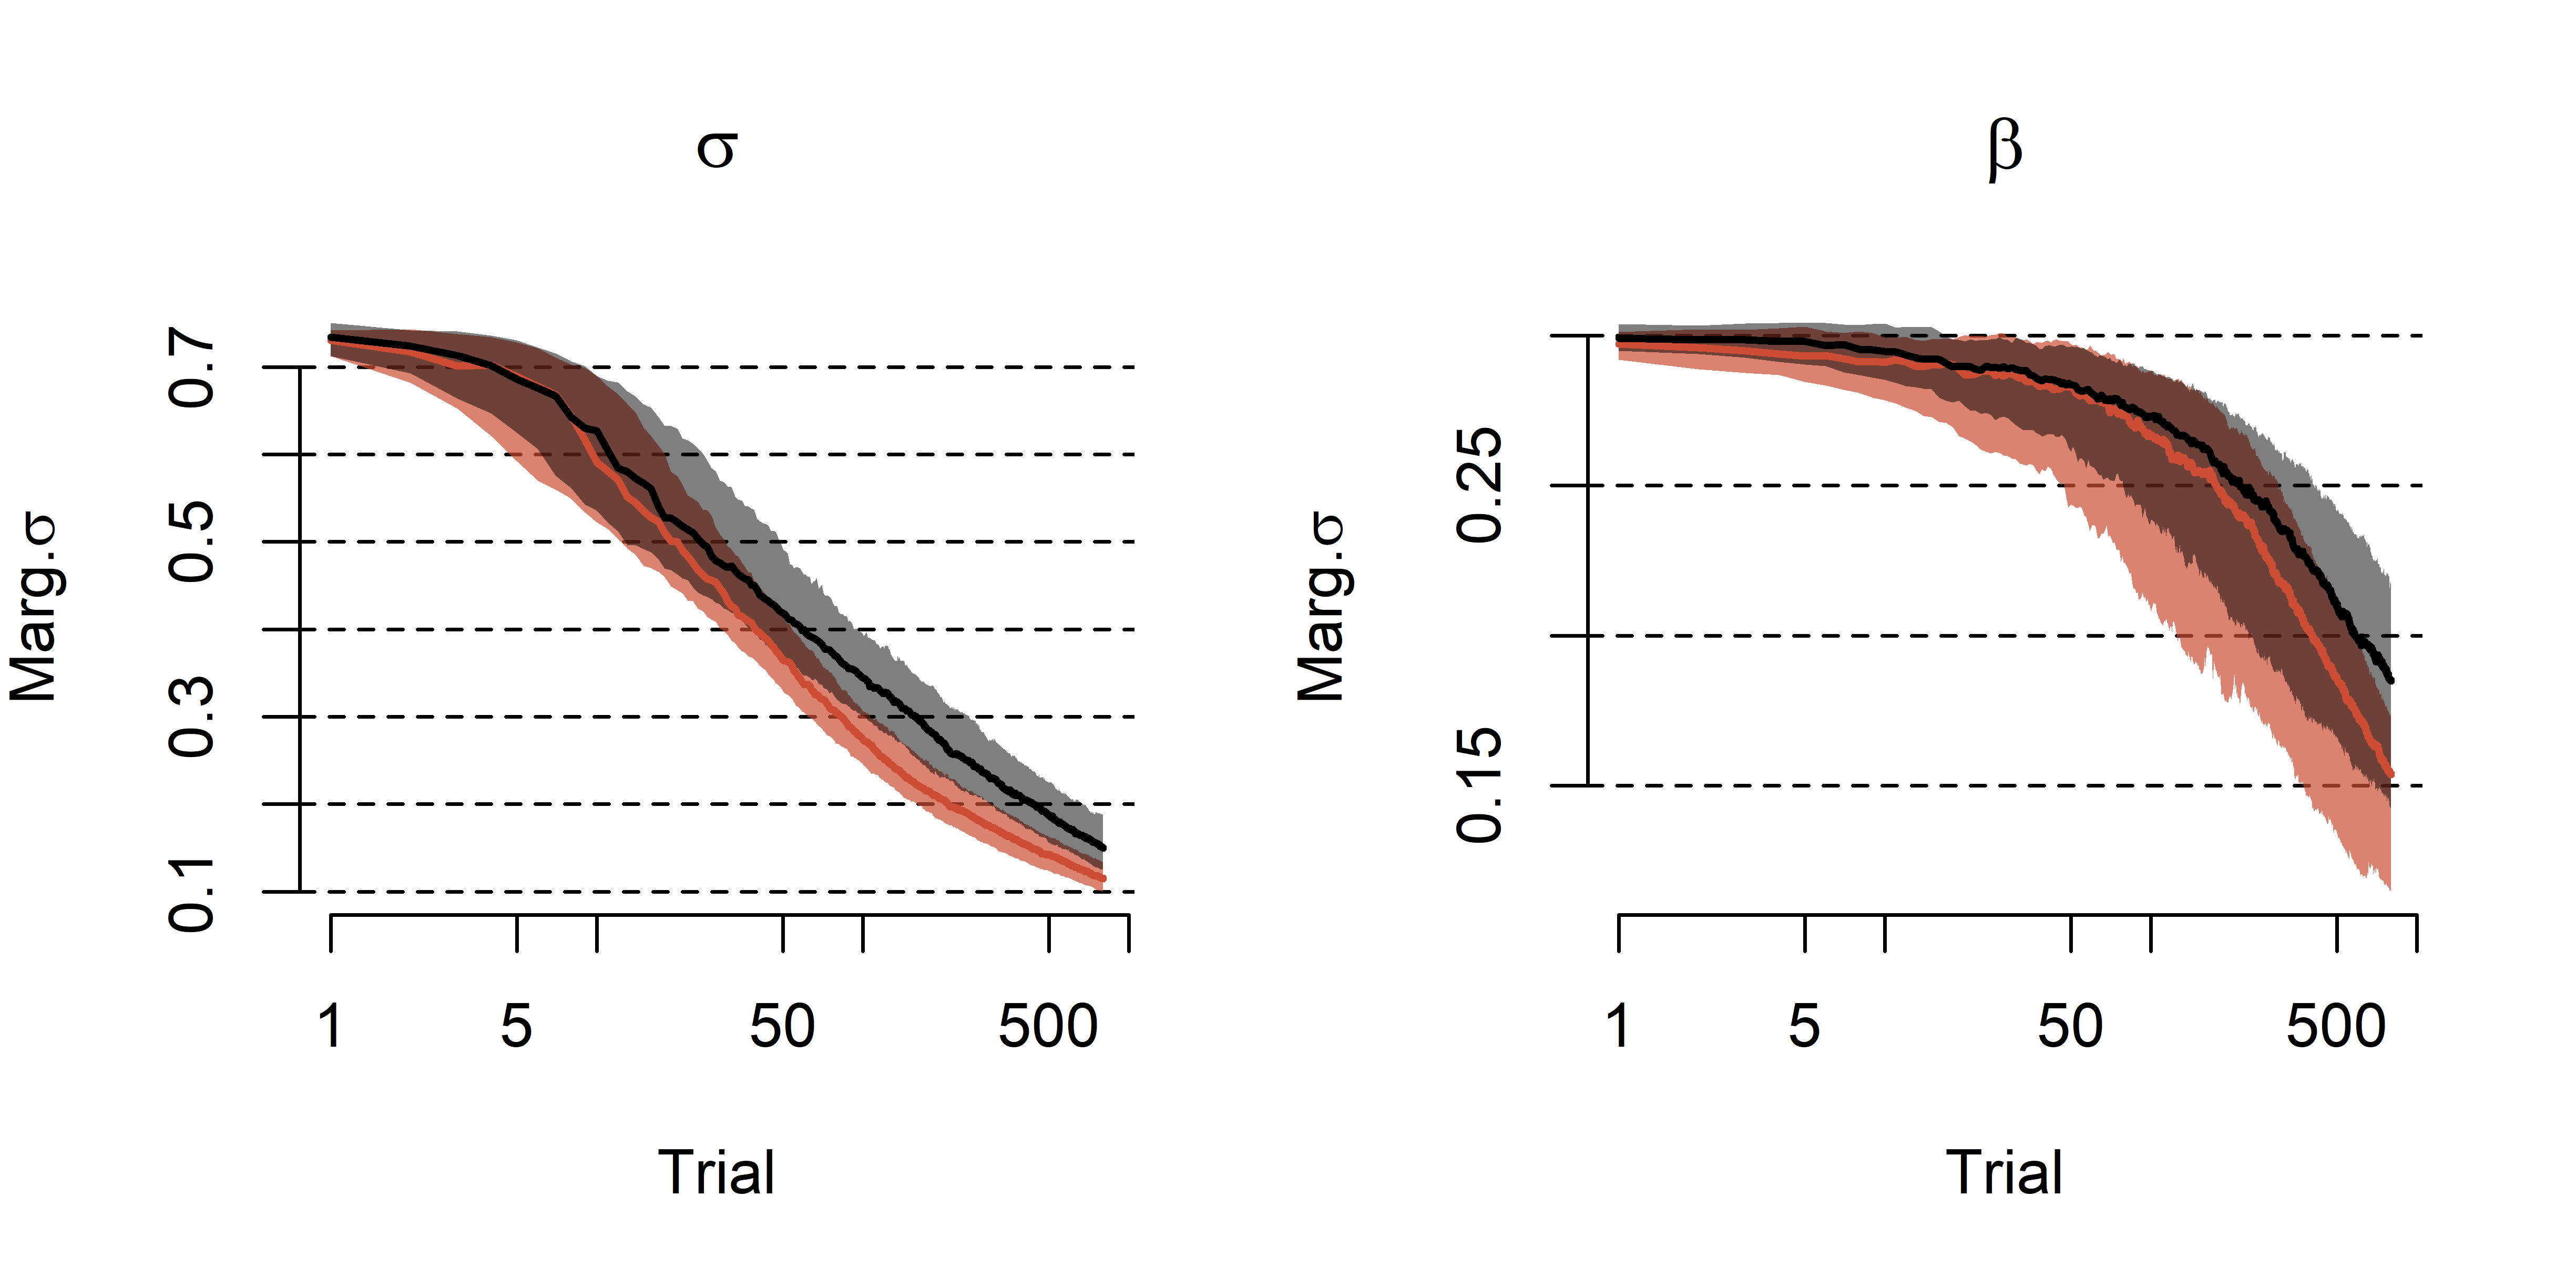
\includegraphics[scale=0.75, angle = 0]{simulation_AFC_sensory_SD}
\caption{Procedure: 2I-4AFC; sensory parameters. Trial-by-trial marginal standard deviations. Red: adaptive algorithm; black: random stimuli.}
\label{fig:simulation_AFC_sensory_SD}
\end{figure}

\begin{figure}[H]
\centering
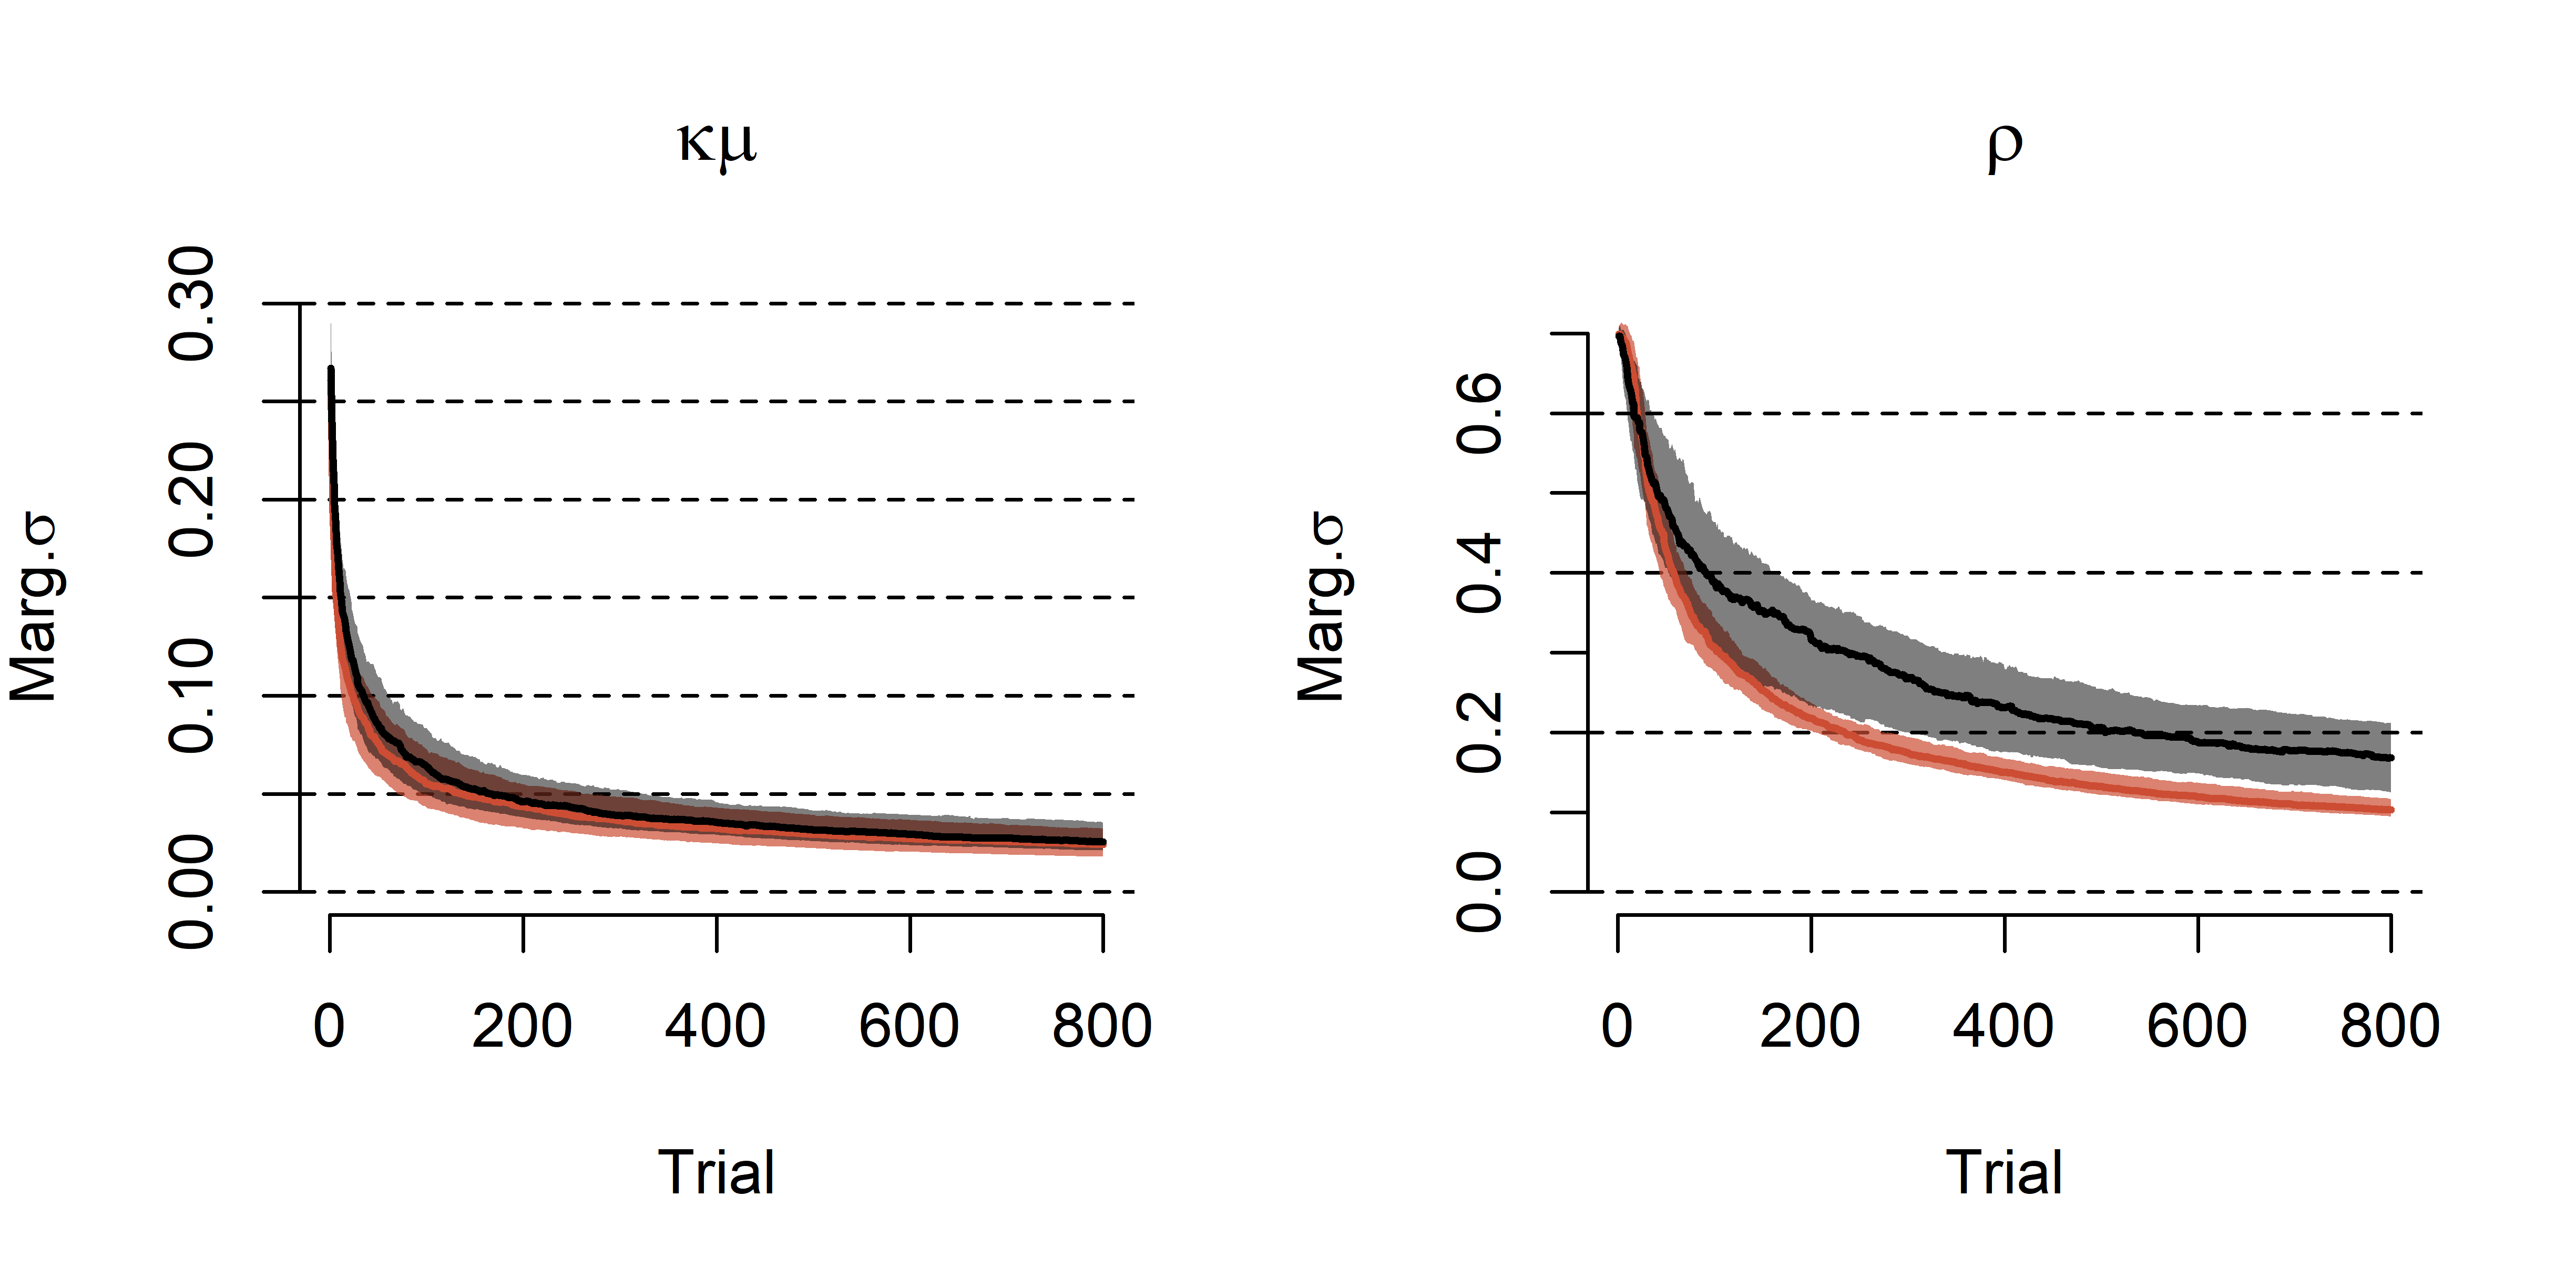
\includegraphics[scale=0.75, angle = 0]{simulation_AFC_interaction_SD}
\caption{Procedure: 2I-4AFC; interaction parameters. Trial-by-trial marginal standard deviations. Red: adaptive algorithm; black: random stimuli.}
\label{fig:simulation_AFC_interaction_SD}
\end{figure}

\paragraph{Hierarchical model}

A hierarchical model was fit to both the marginal standard deviations and squared errors at the last trial to get a more quantitative understanding of the differences at that point. This should be considered as a first-order approximation of a more complete model of performance. Idea behind this approximation is that differences between the algorithms would become more apparent as more trials are completed, and the posterior distribution becomes more dominated by the likelihood; thus the algorithms were compared at the last trial.

A common dummy coded linear model with Gaussian errors was used. The slopes, intercepts and standard deviations were pooled inside each condition, which means that e.g. all of the marginal standard deviations in the Yes/No condition with adaptively selected stimuli were given a common hyperprior. The models were fit using Stan, model code can be found online from \url{https://github.com/joanpaak/ERROR}.

Data was standardized before fitting ($y' = (y - \overline{y}) / \text{SD}(y) $). Parameter-specific $\beta'$ coefficients (slopes fit to standardized data) of the linear model are shown in Figures from \ref{fig:qs_YN_SD} to \ref{fig:qs_AFC_sq_error}. In all plots the thicker parts indicate 50\% and narrower lines 95\% equal-tailed intervals\footnote{\textit{Equal-tailed interval} (ETI) means the interval between some percentiles of the posterior distribution \citep[p. 342]{kruschke2015}, here for example the interval between 2.5\% and 97.5\% for the 95\% ETI.}. Positive values indicate better performance by the adaptive algorithm.

\begin{figure}[H]
\centering
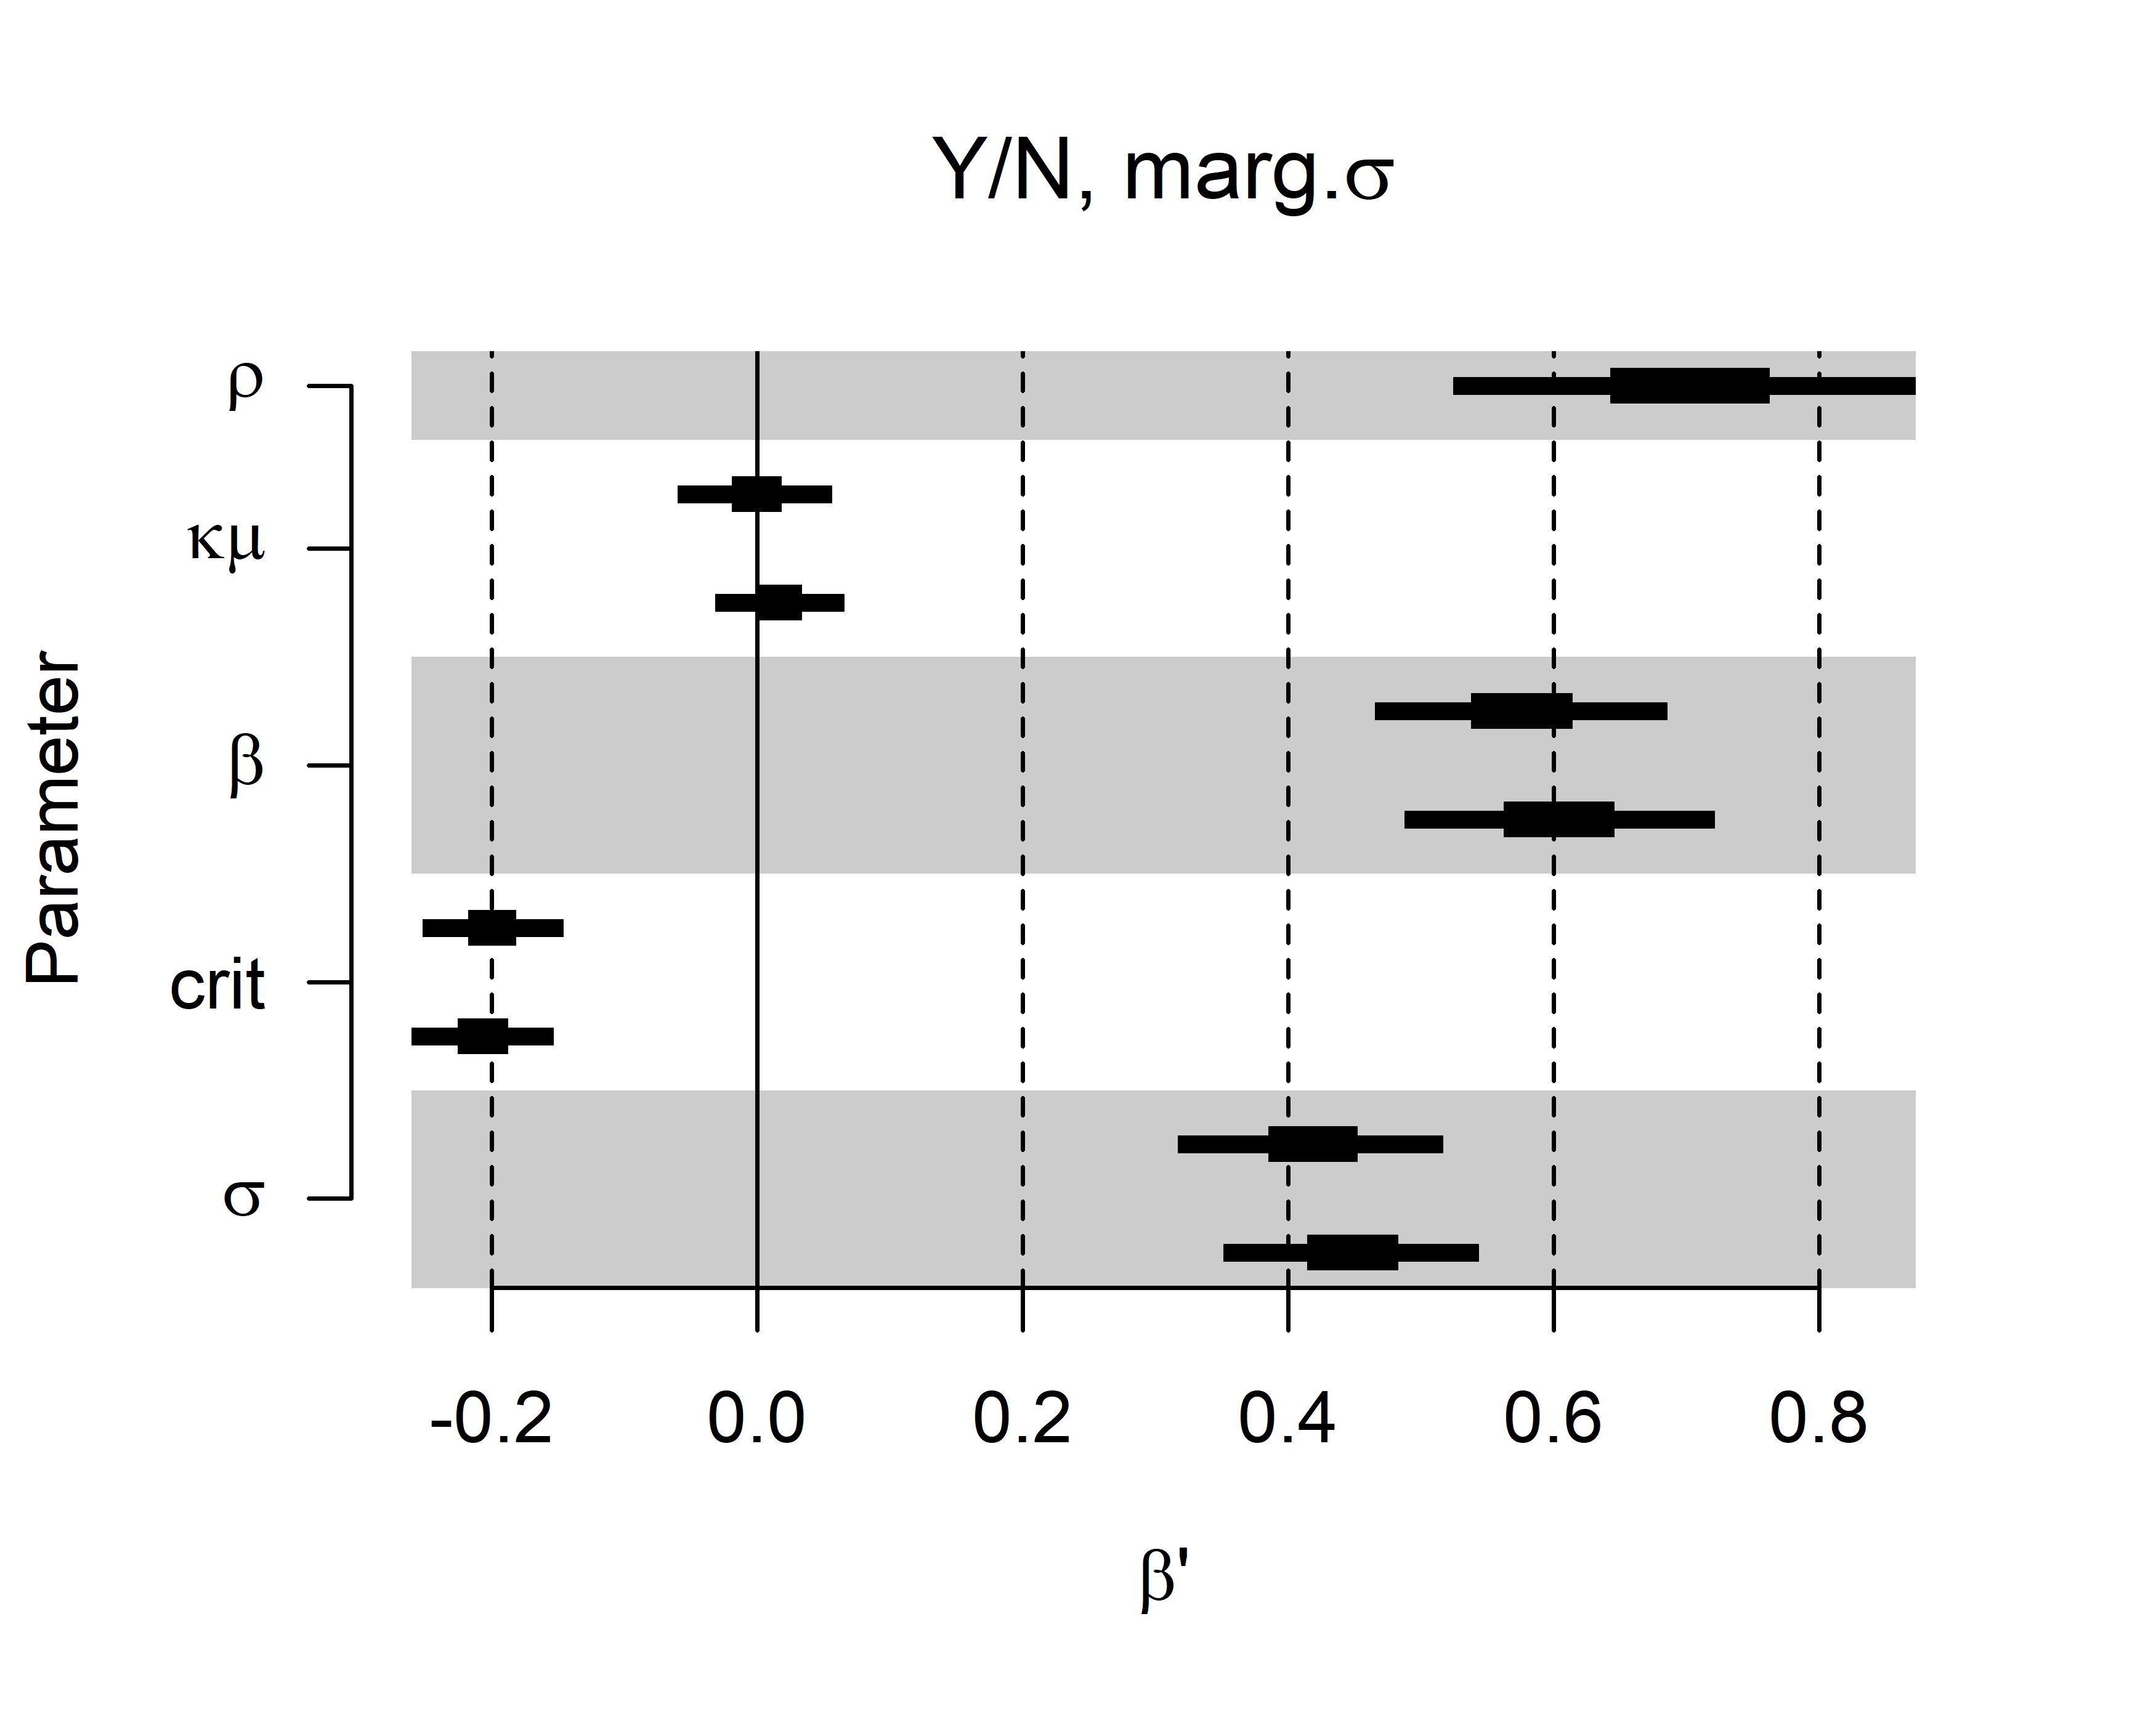
\includegraphics[scale=0.75]{qs_YN_SD}
\caption{Procedure: Yes/No. $\beta'$ coefficients for the difference between adaptive and random algorithms in marginal standard deviations.}
\label{fig:qs_YN_SD}
\end{figure} 

\begin{figure}[H]
\centering
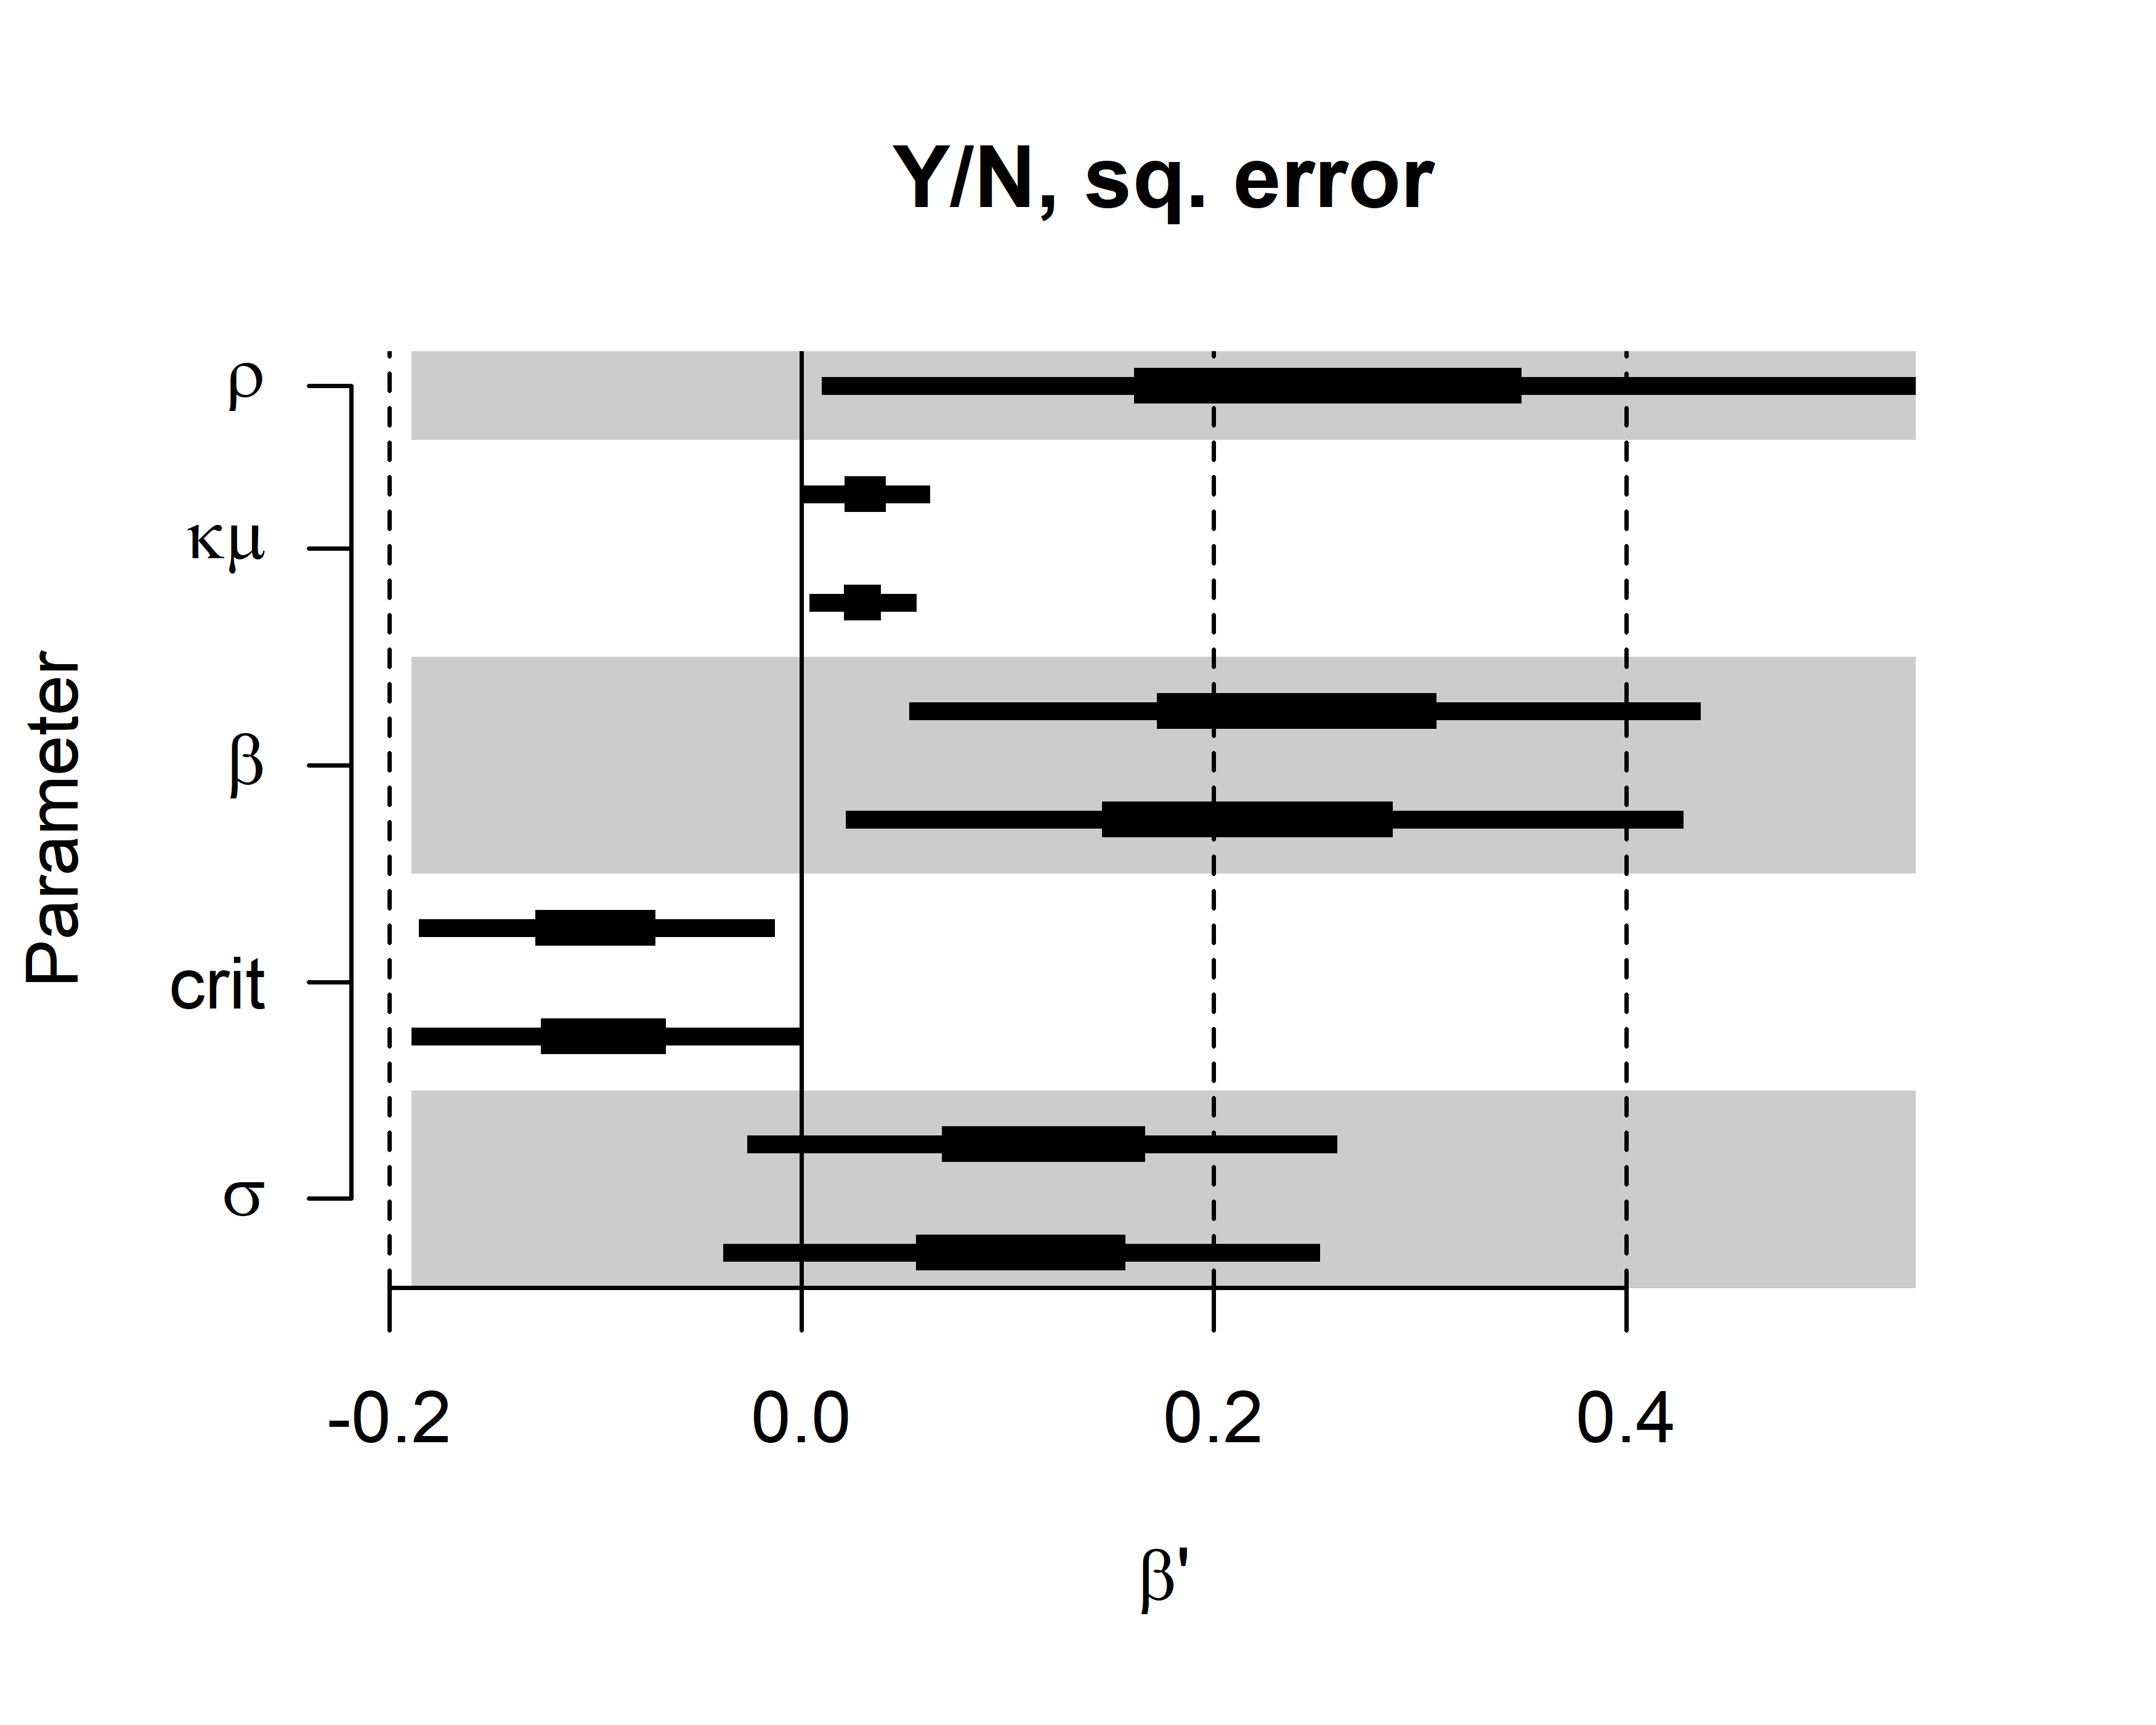
\includegraphics[scale=0.75]{qs_YN_sq_error}
\caption{Procedure: Yes/No. $\beta'$ coefficients for the difference between adaptive and random algorithms in squared errors between marginal means and generating parameters.}
\label{fig:qs_YN_sq_error}
\end{figure} 

\begin{figure}[H]
\centering
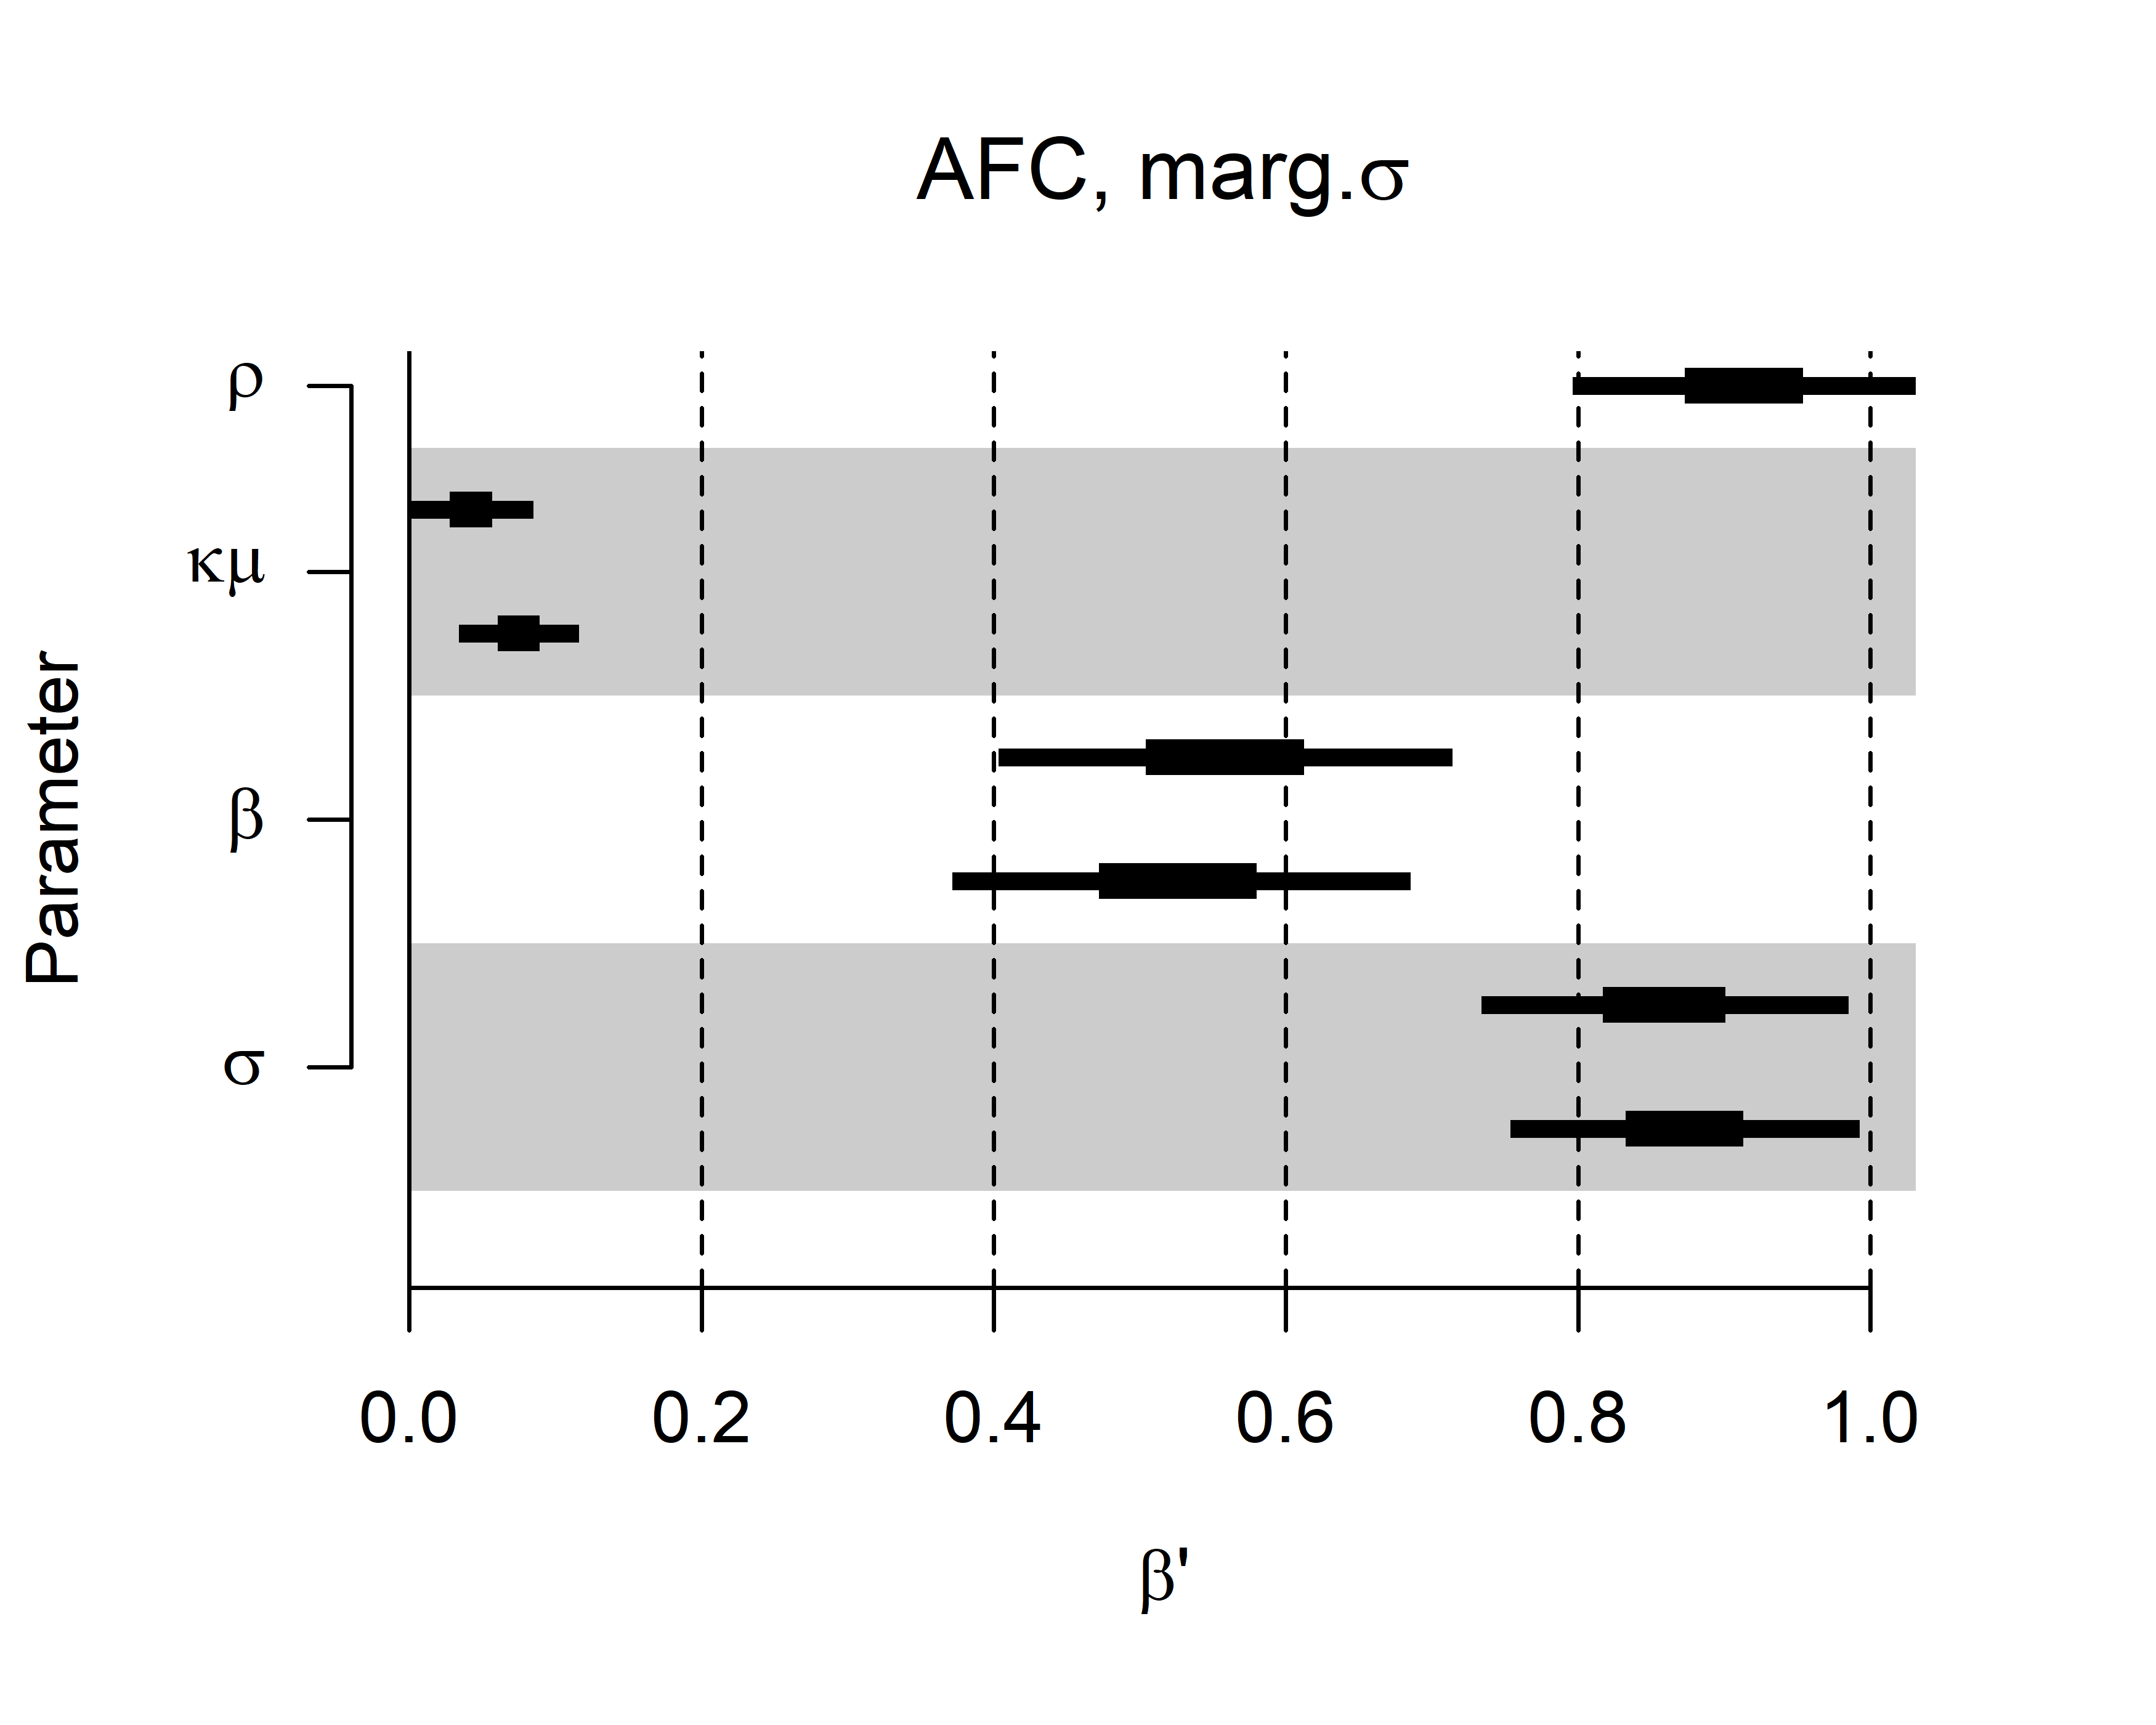
\includegraphics[scale=0.75]{qs_AFC_SD}
\caption{Procedure: 2I-4AFC. $\beta'$ coefficients for the difference between adaptive and random algorithms in marginal standard deviations.}
\label{fig:qs_AFC_SD}
\end{figure} 

\begin{figure}[H]
\centering
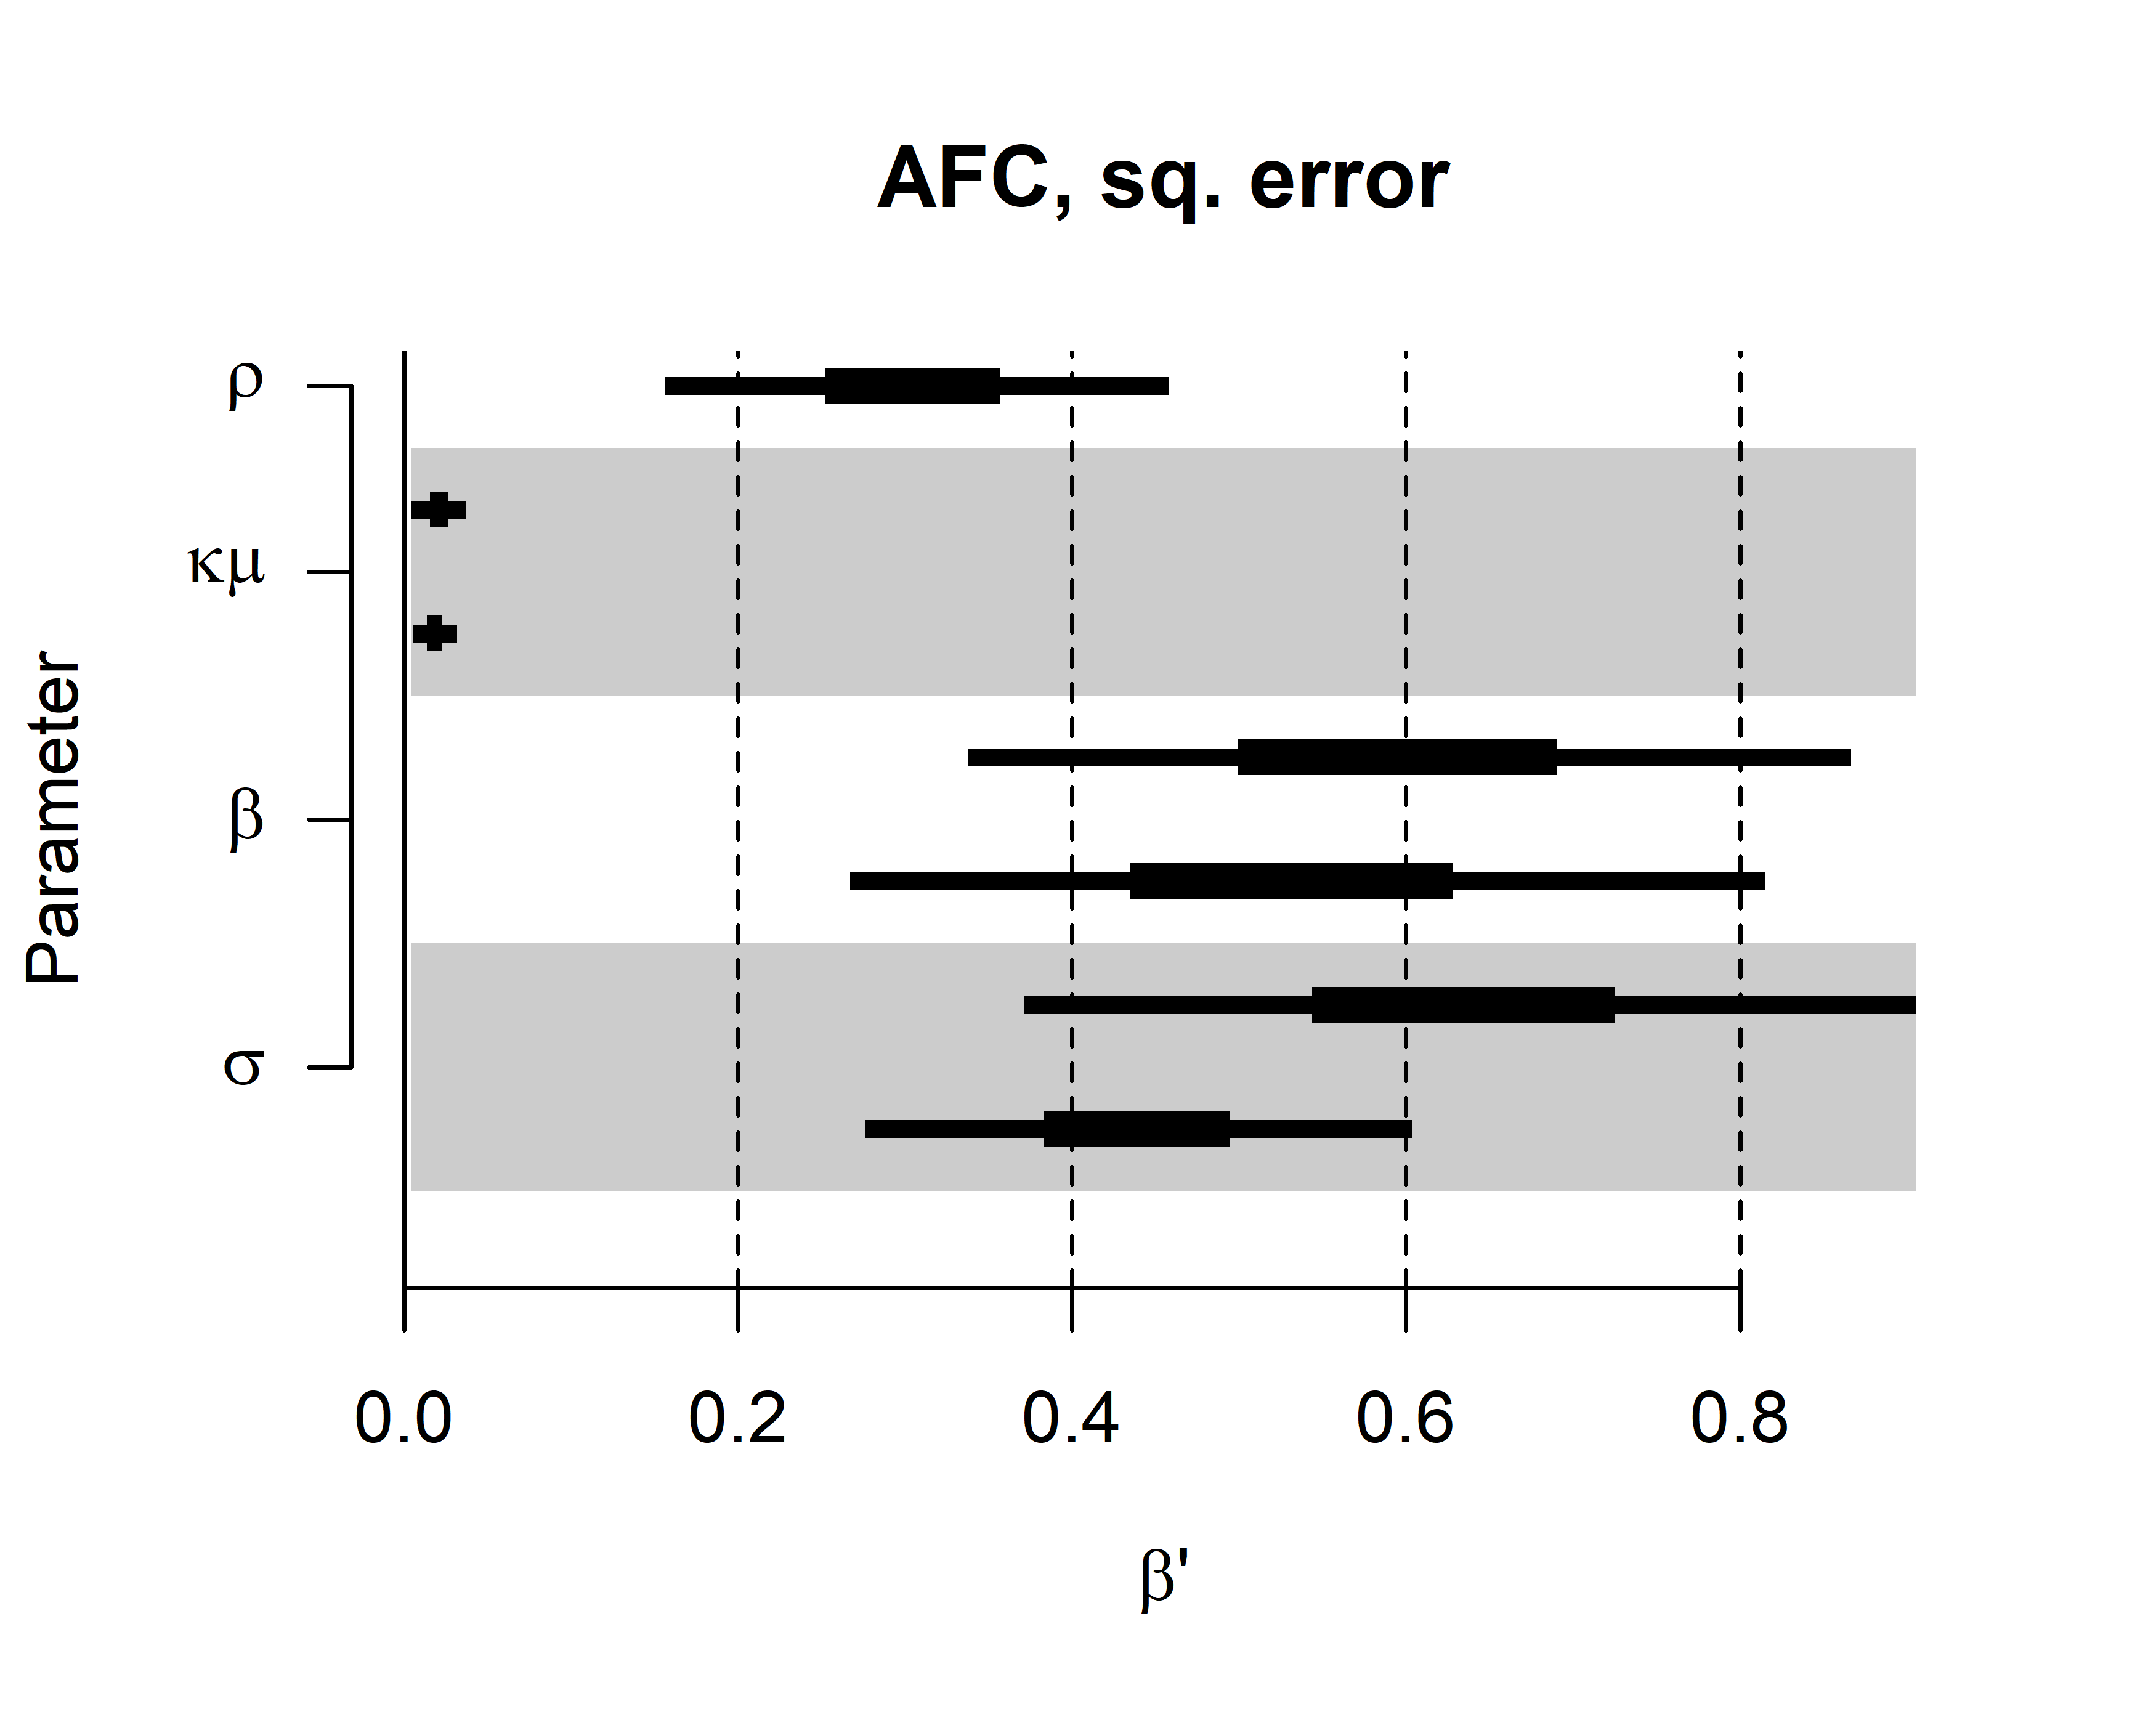
\includegraphics[scale=0.75]{qs_AFC_sq_error}
\caption{Procedure: 2I-4AFC. $\beta'$ coefficients for the difference between adaptive and random algorithms in squared errors between marginal means and generating parameters.}
\label{fig:qs_AFC_sq_error}
\end{figure} 

\subsection{Discussion}

\paragraph{Question 1: is the adaptive algorithm more efficient?}

Judging from Figures \ref{fig:qs_YN_SD} and \ref{fig:qs_AFC_SD}, by the time of 800 completed trials the adaptive algorithm has managed to reduce marginal standard deviations more for parameters $\sigma$, $\beta$ and $\rho$ in both conditions. Effect sizes range from around $0.4$ to almost $1.0$. However, as can be seen from Figures \ref{fig:simulation_YN_sensory_SD}, \ref{fig:simulation_YN_interaction_SD}, \ref{fig:simulation_AFC_sensory_SD} and \ref{fig:simulation_AFC_interaction_SD}, differences in raw scores are fairly modest, around 0.05 to 0.20.

There doesn't seem to be that much difference in $\kappa_{\mu}$ parameters, which is probably explained by the fact that, as can be seen from Figures \ref{fig:simulation_AFC_interaction_SD} and \ref{fig:simulation_YN_interaction_SD} the marginal standard deviations for these parameters reduce fairly quickly.

The most surprising result is that random sampling seems to be more effective in reducing uncertainty about the criteria (Figure \ref{fig:qs_YN_SD}). 

Similar pattern can be observed for the squared errors (Figures \ref{fig:qs_YN_sq_error} and \ref{fig:qs_AFC_sq_error}) but the differences are swamped by a lot more variability. 

\paragraph{Question 2: how well are generating parameters recovered?}

It seems that the majority of of improvement for most parameters happens before 400 trials. After that, information gain seems to slow down considerably.

The most problematic parameters would seem to be the $\beta$ parameters. This contrasts results in for example \cite{kontsevichtyler1999}, and could indicate that when in this more complex model inferences about the non-linearity of the $d'$ function become more uncertain. Note also that the variance of squared error in estimating the $\beta$ parameter increses somewhat during the first 100 trials (Figures \ref{fig:simulation_YN_sensory_sq_error} and \ref{fig:simulation_AFC_sensory_sq_error}, but the effect is more pronounced in the Yes/No condition), implying that for some simulations the posterior means drift further from the generating parameters. 

With regard to the interaction terms, squared errors and marginal standard deviations for the $\kappa_{\mu}$ parameters seem to approach zero fairly quickly, most of the improvements seems to have happened well before 100 trials, but the $\rho$ parameters seem more problematic (Figures \ref{fig:simulation_YN_interaction_sq_error}, \ref{fig:simulation_YN_interaction_SD}, \ref{fig:simulation_AFC_interaction_sq_error} and \ref{fig:simulation_AFC_interaction_SD}). Marginal standard deviations for the $\rho$s don't get, on average, much smaller than $.2$ which still implies a lot of uncertainty--keeping in mind that correlation coefficients are bound between $-1$ and $1$.

\clearpage
\bibliography{references}
\bibliographystyle{apacite}

\end{document}
